\documentclass[12pt]{article}
\usepackage{amssymb}
\usepackage{amsthm}
\usepackage{dsfont}
\usepackage{amsmath}
\usepackage[latin1]{inputenc}
\usepackage[english]{babel}
\usepackage{graphicx}
\usepackage{bbm}
\usepackage{tikz}
\usepackage{color}  
%\usepackage{nath}
%\delimgrowth=1

\usepackage[margin=1in,footskip=0.25in]{geometry}
\linespread{1.3}

\usepackage{verbatim}
\usepackage{enumitem}

\newtheorem{theorem}{Theorem}%[section]
\newtheorem{lemma}[theorem]{Lemma}
\newtheorem{proposition}[theorem]{Proposition}
\newtheorem{corollary}[theorem]{Corollary}
\newtheorem{question}{Open question}
\newtheorem{defi}[theorem]{Definition}
\theoremstyle{plain}
\newtheorem{assumption}{Assumption}

\theoremstyle{remark}
\newtheorem{remark}{Remark}
\newtheorem{example}{\it Example\/}

\theoremstyle{definition}
\newtheorem{exercise}{Exercise}
\newtheorem{problem}{Problem}

\def\RRn{\mathbb{R}^n}
\def\RR{\mathbb{R}}
\def\RRN{\mathbb{R}^N}
\def\ZZ{\mathbb{Z}}
\def\ZZN{\mathbb{Z}^N}
\def\RRnm{\mathbb{R}^{n \times m}}
\def\RRmn{\mathbb{R}^{m \times n}}

\def\dd{\, \mathrm{d}}

\def\grad{\nabla}
\def\weakConv{\rightharpoonup}
\def\LL{\mathrm{L}}
\def\WW{\mathrm{W}}
\def\naturals{\mathbb{N}}

\def\intRRn{\int_{\RRn}}

\def\calM{\mathcal{M}}
\def\calE{\mathcal{E}_p}
\def\calC{\mathcal{C}}

\def\dist{\text{dist}}
\def\supp{\text{supp}}
\def\indyk{\mathds{1}}

\def\intOmega{\int_{\Omega}}
\def\intRRnm{\int_{\RRnm}}

\def\PP{\mathrm{P}}

\def\Ccinfty{C_c^{\infty}}

\DeclareMathOperator{\im}{Im}
\DeclareMathOperator{\id}{Id}
\renewcommand{\phi}{\varphi}
\renewcommand{\epsilon}{\varepsilon}
\renewcommand{\geq}{\geqslant}
\renewcommand{\leq}{\leqslant}
\renewcommand{\div}{\text{div}}

\newcommand{\measurerestr}{%
  \,\raisebox{-.127ex}{\reflectbox{\rotatebox[origin=br]{-90}{$\lnot$}}}\,%
}

\def\Xint#1{\mathchoice
{\XXint\displaystyle\textstyle{#1}}%
{\XXint\textstyle\scriptstyle{#1}}%
{\XXint\scriptstyle\scriptscriptstyle{#1}}%
{\XXint\scriptscriptstyle\scriptscriptstyle{#1}}%
\!\int}
\def\XXint#1#2#3{{\setbox0=\hbox{$#1{#2#3}{\int}$ }
\vcenter{\hbox{$#2#3$ }}\kern-.6\wd0}}
\def\ddashint{\Xint=}
\def\dashint{\Xint-}

\renewcommand{\phi}{\varphi}
\renewcommand{\epsilon}{\varepsilon}
\renewcommand{\geq}{\geqslant}
\renewcommand{\leq}{\leqslant}

\def\RRn{\mathbb{R}^n}
\def\RR{\mathbb{R}}
\def\RRN{\mathbb{R}^N}
\def\ZZ{\mathbb{Z}}
\def\ZZN{\mathbb{Z}^N}
\def\multiindices{\mathbb{Z}^N_+}
\def\RRnm{\mathbb{R}^{n \times m}}
\def\RRmn{\mathbb{R}^{m \times n}}
\def\naturals{\mathbb{N}}

\def\Ccinfty{C_c^{\infty}}

\def\dd{\, \mathrm{d}}
\def\grad{\nabla}
\def\weakConv{\rightharpoonup}

\def\intRRn{\int_{\RRn}}
\def\intOmega{\int_{\Omega}}
\def\intRRnm{\int_{\RRnm}}
\def\intRRN{\int_{\RRN}}

\def\RRNn{\RR^{N \times n}}

\def\CC{\mathrm{C}}

\def\RRn{\RR^n}
\def\RRm{\RR^m}

\usetikzlibrary{shapes, arrows, calc, arrows.meta, fit, positioning}  
\tikzset{  
    -Latex,auto,node distance =1.5 cm and 1.3 cm, thick,
    state/.style ={ellipse, draw, minimum width = 0.9 cm}, 
    point/.style = {circle, draw, inner sep=0.18cm, fill, node contents={}},  
    bidirected/.style={Latex-Latex}, 
    el/.style = {inner sep=2.5pt, align=right, sloped}  
}  

\def\hint{\noindent \textbf{Hint: }}
\begin{document}

\begin{center}
\begin{Large}
\textbf{LN fee bounds}

\end{Large}
\text{sketch}
\end{center}

\begin{itemize}
  \item B - price of 1 on-chain transaction
  \item r - constant effective interest rate
  \item $c_{ij}$ - regular payment from node $i$ to node $j$
  \item $p_{i_{jk}}$ - the fixed transaction fee i charges for each payment from j to k. It could be changed into a function of c
  \item $\lambda_{ij}$ - average transaction frequency between node $i$ and node $j$, (unit: $tx/minute$)
%   \item $\Delta B$ - the rate of change in balance (unit: $token/minute$)
%   \item $\Delta c$ - the number of tokens per combined transaction (unit: $token/tx$)
  \item $m_{ij}$ - channel size between node $i$ and node $j$ (inbound + outbound capacity)
  \item $k$ - the number of intermediate transaction a node can transfer
  \item $\tau(\alpha)$ - an exponential i.i.d. random variable with parameter $\alpha$, indicating the time period $(0,\tau)$ a channel is open 
  \item $T$ - exponential i.i.d random variable with parameter $\alpha$, indicating the total transaction fee charged between $(0,\tau)$
  \item $I$ - exponential i.i.d random variable with parameter $\alpha$, indicating the interest return (opportunity cost) between $(0,\tau)$
  \item $3(\frac{2B\lambda}{r})^{1/3}$ - expected cost of a bidirectional channel (opening, reopening, maintaining)
  \item $\sqrt{\frac{2B\lambda c}{r}}$ - expected cost of an unidirectional channel
  \item $R$ - intermediate node's revenue through transacting payments
\end{itemize}
\section{3 Nodes }
Let there be 1 unidirectional channel between Alice and Bob and 1 bidirectional channel between Bob and Charlie. Let Alice sends payment $c_{AB}$ to Bob at a rate of $\lambda_{AB}$, and Alice wants to send payments of $c_{AC}$ to Charlie at a rate of $\lambda_{AC}$. \\
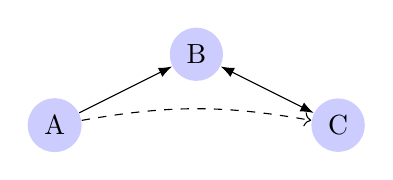
\begin{tikzpicture}  
  [scale=.9,auto=center,every node/.style={circle,fill=blue!20}] 
    
  \node (a1) at (0,0) {A};  
  \node (a2) at (2,1)  {B}; 
  \node (a3) at (4,0)  {C}; 
  
  \path[] (a1) edge[bend left=0]  (a2); 
  \path[bidirected] (a2) edge[bend left=0]  (a3);
  \path[dashed,->] (a1) edge[bend left=10]  (a3); 
\end{tikzpicture} 
% \begin{defi}
%     The model has random variables $\tau$ and $\lambda$. Other parameters are constant. 
% \end{defi}

% Bob can serve as an intermediate node for Alice such that she does not need to create a channel with Charlie. We investigate Bob's cost and fee. 
% \begin{assumption}
%     Bob and Charlie makes more frequent and larger payments with each other, such that Bob is not concerned about the impact Alice's payments has on the channel between him and Charlie.
% \end{assumption}
% Let the size of the channel $AB$ be $m$.
% The net change of balance $\Delta c$ (unit: $token/tx$) for Bob on the channel $AB$ is  
% \begin{align}
%     \Delta c = &c_{AC}/\frac{\lambda_{AC}}{max(\lambda_{AC},\lambda_{AB})}+c_{AB}/\frac{\lambda_{AB}}{max(\lambda_{AC},\lambda_{AB})}+p/\frac{\lambda_{AC}}{max(\lambda_{AC},\lambda_{AB})}
% \end{align}
% \begin{assumption}
%     All the channels have the same $\lambda$.
% \end{assumption}
% Then the number of intermediate transaction $k$ does not depend on $\lambda$. 
% \begin{align}
%     \Delta c& = c_{AC}+c_{AB}+p\\
%     k &= \frac{m}{\Delta c_{AB}} = \frac{m}{c_{AC}+c_{AB}+p}
% \end{align}

% Then we find the amount of time the channel $AB$ is open in terms of $\lambda$s. 

% The rate of change in balance $\Delta B$ (unit: $token/minute$) of the channel $AB$ is 
% \begin{align}
%     \Delta B &= c_{AC}\lambda_{AC}+c_{AB}\lambda_{AB}+p\lambda_{AC} = (c_{AC}+c_{AB}+p)\lambda
% \end{align}

% Hence, the time a channel is open is 
% \begin{align}
%     \tau = \frac{m}{\Delta B} = \frac{m}{c_{AC}\lambda_{AC}+c_{AB}\lambda_{AB}+p\lambda_{AC}}=\frac{m}{(c_{AC}+c_{AB}+p)\lambda}
% \end{align}
% \begin{remark}
%     $\lambda$ is a random variable depended on $\tau$. However, since $\lambda$ is not involved with the later calculations, we will not calculate its value and assume that it is some appropriate function of $\tau$. 
% \end{remark}

% \subsection{Interest return gain in bank}

% By storing $\frac{c}{e^{r\tau}}$ in the bank at time $t=0$, the balance grow to $c$ at time $t=\tau$. If a node store $c$ in the channel, then assuming they do not change the balance, then they get $c$ back when the channel closes.\\
% The cost to store $c$ in a channel that opens during the time $(0,\tau)$, is 
% \begin{align}
%     I_1 &= c-ce^{-r\tau}
% \end{align}
% Then the expected interest return of a channel is 
% \begin{align}
%     I(\alpha) = E[I_1] &= c-cE[e^{-r\tau}] = c-c\frac{\alpha}{\alpha + r}
% \end{align}

% \subsection{Transaction fee}
% Recall the number of transactions Bob can handle is $k = \frac{m}{\Delta c}=\frac{m}{c+c_{AB}+p}$. 
% \begin{assumption}
%     Bob charges a constant fee $p$ for each transaction
% \end{assumption}
% For the entirety of the channel, Bob will gain transaction fee
% \begin{align}
%     T_1 = p\cdot k \cdot e^{-r\tau}
% \end{align}
The expected interest return of a channel $I$ and the transaction fee are 
\begin{align}
    I(\alpha) &= c-c\frac{\alpha}{\alpha + r}\\
    T(\alpha) &= \frac{mp}{c_{AC}+c_{AB}+p} \cdot \frac{\alpha}{\alpha + r}
\end{align}
We try to find the bounds of the fixed payment p. 
\subsubsection{With optimal channel size}
The optimal size of the channel is $m=\sqrt{\frac{2B\lambda c}{r}}$. Here, $c=c_{AC}+c_{AB}+p$, such that $m=\sqrt{\frac{2B\lambda (c_{AC}+c_{AB}+p)}{r}}$. Note that both $2B\lambda (c_{AC}+c_{AB}+p)\geq 0$ and $r> 0$.
\\ Thus transaction fee with the channel having an optimal channel size is 
\begin{align}
    T(\alpha) &= \frac{p\alpha}{(c_{AC}+c_{AB}+p)(\alpha+r)} \cdot \sqrt{\frac{2B\lambda (c_{AC}+c_{AB}+p)}{r}}\\
    & = \frac{p\alpha}{(\alpha+r)} \cdot \sqrt{\frac{2B\lambda }{(c_{AC}+c_{AB}+p)r}}
\end{align}

\subsection{Lower bound}
As an intermediate node, Bob is rational to save extra tokens if profit from transaction fees in the node is at least as high as the interest returns if the tokens were saved in a bank. He can also be incentivized to be an intermediate node if their channel capacities becomes unbalanced. With only 2 channels, we don't consider the rebalancing case.
\\ Bob consider the net change in the cost of channels, let $C_o$ be the total cost for old channels, $C_n$ be the total cost for new channels, and sub-subscript $i$ indicates the portion $i$ pays. 
\\ His revenue is bounded below by 0, since he will not agree to be an intermediate node otherwise. 
\begin{align}
  R(\lambda,\alpha) & =T(\alpha) + C_{o_B}(\lambda) - I(\alpha) - C_{n_B}(\lambda)\geq 0\\
  T(\lambda) & \geq  I(\lambda) + C_{n_B}(\lambda) - C_{o_B}(\lambda)
\end{align}
Without Alice's payments to Charlie, each node is responsible for half of the cost to maintain their channels, and thus their costs of the channels is
\begin{align}
  C_{o}(\lambda)&=\sqrt{\frac{2B\lambda c_{AB}}{r}} + 3(\frac{2B\lambda}{r})^{1/3}\\
  C_{o_B}(\lambda)&=\frac{1}{2}\sqrt{\frac{2B\lambda c_{AB}}{r}} + \frac{3}{2}(\frac{2B\lambda}{r})^{1/3}\\
  C_{o_A}(\lambda)&=\frac{1}{2}\sqrt{\frac{2B\lambda c_{AB}}{r}}\\
  C_{o_C}(\lambda) &= \frac{3}{2}(\frac{2B\lambda}{r})^{1/3}
\end{align}
Bob acting as an intermediate node causes him to be responsible for the new frequency $\lambda_{AC}=\lambda$, such that Bob is forced to send transactions as often as necessary. 
\\ The new cost of the channels are 
\begin{align}
  C_{n}(\lambda)&=\sqrt{\frac{2B\lambda (c_{AB}+ c_{AC})}{r}} + 3(\frac{4B\lambda}{r})^{1/3}\\
  C_{n_A}(\lambda)&=C_{o_A}(\lambda) \\
  C_{n_C}(\lambda)&= C_{o_C}(\lambda)\\
  C_{n_B}(\lambda)&=C_{n}(\lambda)-C_{n_A}(\lambda)-C_{n_C}(\lambda) \\
  & = \sqrt{\frac{2B\lambda (c_{AB}+ c_{AC})}{r}} + 3(\frac{4B\lambda}{r})^{1/3} - \frac{1}{2}\sqrt{\frac{2B\lambda c_{AB}}{r}}- \frac{3}{2}(\frac{2B\lambda}{r})^{1/3}
\end{align}
From the earlier secions, we have 
\begin{align}
  I(\alpha) &= c_{AC}-c_{AC}\frac{\alpha}{\alpha + r}\\
  T(\alpha) &= \frac{mp}{c_{AC}+c_{AB}+p} \cdot \frac{\alpha}{\alpha + r}
\end{align}
Plugging these equations in
\begin{align}
  T(\alpha) & \geq  I(\alpha) + C_{n_B}(\lambda) - C_{o_B}(\lambda)\\
  \frac{mp}{c_{AC}+c_{AB}+p} \cdot \frac{\alpha}{\alpha + r} & \geq \frac{c_{AC}r}{\alpha + r} + \sqrt{\frac{2B\lambda (c_{AB}+ c_{AC})}{r}}\\
  &  + 3(\frac{4B\lambda}{r})^{1/3} - \sqrt{\frac{2B\lambda c_{AB}}{r}}- 3(\frac{2B\lambda}{r})^{1/3}
\end{align}
We find the lower bound for $p$
\begin{align}
  &\frac{mp}{c_{AC}+c_{AB}+p} \geq \frac{c_{AC}r}{\alpha} + \frac{\alpha + r}{\alpha}(((c_{AB}+ c_{AC})^{1/2}-c_{AB}^{1/2})\sqrt{\frac{2B\lambda }{r}}\\
  &  + 3(4^{1/3}-2^{1/3})(\frac{B\lambda}{r})^{1/3})\\
  p & \geq \frac{(c_{AC}+c_{AB})(\frac{c_{AC}r}{\alpha} + \frac{\alpha + r}{\alpha}((\sqrt{c_{AB}+ c_{AC}}-\sqrt{c_{AB}})\sqrt{\frac{2B\lambda }{r}} + 3(4^{1/3}-2^{1/3})(\frac{B\lambda}{r})^{1/3}))}{m-(\frac{c_{AC}r}{\alpha} + \frac{\alpha + r}{\alpha}(((c_{AB}+ c_{AC})^{1/2}-c_{AB}^{1/2})\sqrt{\frac{2B\lambda }{r}} + 3(4^{1/3}-2^{1/3})(\frac{B\lambda}{r})^{1/3}))}
\end{align}
The optimal size of the channel is $m=\sqrt{\frac{2B\lambda c}{r}}$. Here, $c=c_{AC}+c_{AB}+p$, such that $m=\sqrt{\frac{2B\lambda (c_{AC}+c_{AB}+p)}{r}}$. The lower bound with this size of the channel is 
\begin{align}
  p & \geq \frac{(c_{AC}+c_{AB})(\frac{c_{AC}r}{\alpha} + \frac{\alpha + r}{\alpha}((\sqrt{c_{AB}+ c_{AC}}-\sqrt{c_{AB}})\sqrt{\frac{2B\lambda }{r}} + 3(4^{1/3}-2^{1/3})(\frac{B\lambda}{r})^{1/3}))}{\sqrt{\frac{2B\lambda (c_{AC}+c_{AB}+p)}{r}}-(\frac{c_{AC}r}{\alpha} + \frac{\alpha + r}{\alpha}(((c_{AB}+ c_{AC})^{1/2}-c_{AB}^{1/2})\sqrt{\frac{2B\lambda }{r}} + 3(4^{1/3}-2^{1/3})(\frac{B\lambda}{r})^{1/3}))}\\
  p & \geq \frac{(c_{AC}+c_{AB})(c_{AC}r + (\alpha + r)((\sqrt{c_{AB}+ c_{AC}}-\sqrt{c_{AB}})\sqrt{\frac{2B\lambda }{r}} + 3(4^{1/3}-2^{1/3})(\frac{B\lambda}{r})^{1/3}))}{\alpha\sqrt{\frac{2B\lambda (c_{AC}+c_{AB}+p)}{r}}-(c_{AC}r + (\alpha + r)(((c_{AB}+ c_{AC})^{1/2}-c_{AB}^{1/2})\sqrt{\frac{2B\lambda }{r}} + 3(4^{1/3}-2^{1/3})(\frac{B\lambda}{r})^{1/3}))}
%   &\alpha p\frac{\sqrt{\frac{2B\lambda (c_{AC}+c_{AB}+p)}{r}}}{(c_{AC}r + (\alpha + r)(((c_{AB}+ c_{AC})^{1/2}-c_{AB}^{1/2})\sqrt{\frac{2B\lambda }{r}} + 3(4^{1/3}-2^{1/3})(\frac{B\lambda}{r})^{1/3}))}-\alpha p\\
%   & \geq (c_{AC}+c_{AB})\\
%   &\alpha p\sqrt{\frac{2B\lambda (c_{AC}+c_{AB}+p)}{r}}-\alpha p(c_{AC}r + (\alpha + r)(((c_{AB}+ c_{AC})^{1/2}-c_{AB}^{1/2})\sqrt{\frac{2B\lambda }{r}} + 3(4^{1/3}-2^{1/3})(\frac{B\lambda}{r})^{1/3}))\\
%   & \geq (c_{AC}+c_{AB})(c_{AC}r + (\alpha + r)(((c_{AB}+ c_{AC})^{1/2}-c_{AB}^{1/2})\sqrt{\frac{2B\lambda }{r}} + 3(4^{1/3}-2^{1/3})(\frac{B\lambda}{r})^{1/3}))
\end{align}


\subsection{Upper bound}
The intermediate nodes must keep their fee at most the cost of their clients to use on-chain transactions (either to make transactions, or open, reopen, or update the channel) or to create a direct channel with the destined node. 
\\ Alice analyze when will it be beneficial for her to open a direct channel with Charlie, or pay for Bob's service. 
\\ If Alice creates a direct unidirectional channel with Charlie, Bob's cost of channels doesn't change, while Alice and Charlie has a different cost from the previous section. 
\begin{align}
  C_{o_B}(\lambda)&=C_{n_B}(\lambda)=\frac{1}{2}\sqrt{\frac{2B\lambda c_{AB}}{r}} + \frac{3}{2}(\frac{2B\lambda}{r})^{1/3}\\
  C_{o_A}(\lambda)&=\frac{1}{2}\sqrt{\frac{2B\lambda c_{AB}}{r}}+\frac{1}{2}\sqrt{\frac{2B\lambda c_{AC}}{r}}\\
  C_{o_C}(\lambda) &= \frac{3}{2}(\frac{2B\lambda}{r})^{1/3}+\frac{1}{2}\sqrt{\frac{2B\lambda c_{AC}}{r}}
\end{align}
Collectively, Alice and Charlie pays 
\begin{align}
  C_{o_{AC}}(\lambda) & = \frac{1}{2}\sqrt{\frac{2B\lambda c_{AB}}{r}}+ \frac{3}{2}(\frac{2B\lambda}{r})^{1/3}+\sqrt{\frac{2B\lambda c_{AC}}{r}}
\end{align}
If Alice and Charlie uses Bob's service, their cost of payment is 
\begin{align}
  C_{n_A}(\lambda)&=\frac{1}{2}\sqrt{\frac{2B\lambda c_{AB}}{r}}\\
  c_{n_C}(\lambda) & =\frac{3}{2}(\frac{2B\lambda}{r})^{1/3} \\
  C_{n_{AC}}(\lambda)&=\frac{1}{2}\sqrt{\frac{2B\lambda c_{AB}}{r}}+\frac{3}{2}(\frac{2B\lambda}{r})^{1/3} 
\end{align}
regardless of who actually pays, their maximum willingness to pay is bounded by the change in cost of channels, which is simply the cost of the new channel. 
\begin{align}
  C_{o_{AC}}(\lambda) &\geq C_{n_{AC}}(\lambda) + T(\lambda)\\
  T(\lambda) &\leq C_{o_{AC}}(\lambda) - C_{n_{AC}}(\lambda)\\
  \frac{mp}{c_{AC}+c_{AB}+p} \cdot \frac{\alpha}{\alpha + r} &\leq  \sqrt{\frac{2B\lambda c_{AC}}{r}}
\end{align}
Thus the bound of $p$ is 
\begin{align}
  p &\leq  \frac{(c_{AC}+c_{AB})\sqrt{\frac{2B\lambda c_{AC}}{r}}\frac{\alpha + r}{\alpha}}{m-\sqrt{\frac{2B\lambda c_{AC}}{r}}\frac{\alpha + r}{\alpha}}
\end{align}
With the optimial channel size $m=\sqrt{\frac{2B\lambda (c_{AC}+c_{AB}+p)}{r}}$, the upper bound becomes
\begin{align}
  p &\leq  \frac{(c_{AC}+c_{AB})\sqrt{\frac{2B\lambda c_{AC}}{r}}\frac{\alpha + r}{\alpha}}{\sqrt{\frac{2B\lambda (c_{AC}+c_{AB}+p)}{r}}-\sqrt{\frac{2B\lambda c_{AC}}{r}}\frac{\alpha + r}{\alpha}}\\
  p &\leq  \frac{(c_{AC}+c_{AB})\sqrt{c_{AC}}(\alpha + r)}{\alpha\sqrt{(c_{AC}+c_{AB}+p)}-\sqrt{c_{AC}}(\alpha + r)}
\end{align}
% To analyze if it is beneficial to use indirect transfers, the intermediate nodes must charge between the bounds. When will the bounds be possible?
% \begin{align}
%   &
% \end{align}
% If $\frac{c^2\lambda^{2/3}}{mr^{2/3}B^{1/3}} \leq .5244$, then it is possible for Bob to charge a fee that satifies both the lower bound and upper bound, which leads to a feasible routing from Alice to Charlie.
% \\ If $\frac{c^2\lambda^{2/3}}{mr^{2/3}B^{1/3}} > .5244$, then there is no possible value of transaction fees for the routing to be beneficial for both of the intermediate nodes and the end nodes. 
% \\ Fixing $c, m, r, B$, observe that as $\lambda$ increase, the bounds of the transaction fee shifts to the left, and the lower bound shifts less than the shift of upper bound, thus the maximum benefit of senders and reciever (Alice and Charlie) get from the route decreases more than the benefit of intermediate node (Bob). 

% \subsection{portion of payments}
% The bounds for $p$ are
% \begin{align}
%   & \frac{(c_{AC}+c_{AB})\sqrt{\frac{2B\lambda c_{AC}}{r}}\frac{\alpha + r}{\alpha}}{m-\sqrt{\frac{2B\lambda c_{AC}}{r}}\frac{\alpha + r}{\alpha}}\geq \\
%   p & \geq \frac{(c_{AC}+c_{AB})(\frac{c_{AC}r}{\alpha} + \frac{\alpha + r}{\alpha}((\sqrt{c_{AB}+ c_{AC}}-\sqrt{c_{AB}})\sqrt{\frac{2B\lambda }{r}} + 3(4^{1/3}-2^{1/3})(\frac{B\lambda}{r})^{1/3}))}{m-(\frac{c_{AC}r}{\alpha} + \frac{\alpha + r}{\alpha}(((c_{AB}+ c_{AC})^{1/2}-c_{AB}^{1/2})\sqrt{\frac{2B\lambda }{r}} + 3(4^{1/3}-2^{1/3})(\frac{B\lambda}{r})^{1/3}))}
% \end{align}
% We observe how the bounds change with $c_{AC}$ in relation to $c_{AB}$. 
% \begin{assumption}
%   $c = c_{AC} = c_{AB} $
% \end{assumption}
% The bounds are 
% \begin{align}
%   & \frac{2c\sqrt{\frac{2B\lambda c}{r}}\frac{\alpha + r}{\alpha}}{m-\sqrt{\frac{2B\lambda c}{r}}\frac{\alpha + r}{\alpha}}\geq 
%   p  \geq \frac{(2c)(\frac{cr}{\alpha} + \frac{\alpha + r}{\alpha}((\sqrt{2c}-\sqrt{c})\sqrt{\frac{2B\lambda }{r}} + 3(4^{1/3}-2^{1/3})(\frac{B\lambda}{r})^{1/3}))}{m-(\frac{cr}{\alpha} + \frac{\alpha + r}{\alpha}(((2c)^{1/2}-c^{1/2})\sqrt{\frac{2B\lambda }{r}} + 3(4^{1/3}-2^{1/3})(\frac{B\lambda}{r})^{1/3}))}
% \end{align}





\section{Simplifying the bounds}
With optimal channel size, and assume that all the $c$'s are 1. The bounds of p are 
\begin{align}
    &\frac{(c_{AC}+c_{AB})(c_{AC}r + (\alpha + r)((\sqrt{c_{AB}+ c_{AC}}-\sqrt{c_{AB}})\sqrt{\frac{2B\lambda }{r}} + 3(4^{1/3}-2^{1/3})(\frac{B\lambda}{r})^{1/3}))}{\alpha\sqrt{\frac{2B\lambda (c_{AC}+c_{AB}+p)}{r}}-(c_{AC}r + (\alpha + r)(((c_{AB}+ c_{AC})^{1/2}-c_{AB}^{1/2})\sqrt{\frac{2B\lambda }{r}} + 3(4^{1/3}-2^{1/3})(\frac{B\lambda}{r})^{1/3}))}\\
    &\leq p \leq  \frac{(c_{AC}+c_{AB})\sqrt{c_{AC}}(\alpha + r)}{\alpha\sqrt{(c_{AC}+c_{AB}+p)}-\sqrt{c_{AC}}(\alpha + r)}\\
    \Rightarrow &\frac{2(r + (\alpha + r)((\sqrt{2}-1)\sqrt{\frac{2B\lambda }{r}} + 3(4^{1/3}-2^{1/3})(\frac{B\lambda}{r})^{1/3}))}{\alpha\sqrt{\frac{2B\lambda (2+p)}{r}}-(r + (\alpha + r)((\sqrt{2}-1)\sqrt{\frac{2B\lambda }{r}} + 3(4^{1/3}-2^{1/3})(\frac{B\lambda}{r})^{1/3}))} \\
    & \leq p \leq  \frac{2\alpha + 2r}{\alpha\sqrt{2+p}-\alpha - r}
\end{align}
Simplifying the lower bound
\begin{align}
    &2r + 2(\alpha + r)(\sqrt{2}-1)\sqrt{\frac{2B\lambda }{r}} +  2(\alpha + r)3(4^{1/3}-2^{1/3})(\frac{B\lambda}{r})^{1/3} \leq \\
    &p\alpha\sqrt{\frac{2B\lambda (2+p)}{r}}- pr -p (\alpha + r)(\sqrt{2}-1)\sqrt{\frac{2B\lambda }{r}}-p (\alpha + r) 3(4^{1/3}-2^{1/3})(\frac{B\lambda}{r})^{1/3}\\
    % \Rightarrow &2r + (\alpha + r)(4-2\sqrt{2})\sqrt{\frac{B\lambda }{r}} +  (\alpha + r)(6\cdot 4^{1/3}-6 \cdot 2^{1/3})(\frac{B\lambda}{r})^{1/3} \leq \\
    % &p\alpha\sqrt{\frac{4B\lambda+2B\lambda p}{r}}- pr -p (\alpha + r)(2-\sqrt{2})\sqrt{\frac{B\lambda }{r}}-p (\alpha + r) (3\cdot 4^{1/3}-3\cdot 2^{1/3})(\frac{B\lambda}{r})^{1/3}\\
    \Rightarrow &2r + 1.17157(\alpha + r)\sqrt{\frac{B\lambda }{r}} +  1.96488(\alpha + r)(\frac{B\lambda}{r})^{1/3} \leq \\
    &p\alpha\sqrt{\frac{4B\lambda+2B\lambda p}{r}}- pr -.585786p (\alpha + r)\sqrt{\frac{B\lambda }{r}}-.98244p (\alpha + r) (\frac{B\lambda}{r})^{1/3}\\
    \Rightarrow &2r + 1.17157(\alpha + r)\sqrt{\frac{B\lambda }{r}} +  1.96488(\alpha + r)(\frac{B\lambda}{r})^{1/3} \leq \\
    &p\alpha\sqrt{\frac{4B\lambda+2B\lambda p}{r}}- pr -.585786p (\alpha + r)\sqrt{\frac{B\lambda }{r}}-.98244p (\alpha + r) (\frac{B\lambda}{r})^{1/3}\\
    % \Rightarrow &(2+p)r + (1.17157+.585786p)(\alpha + r)\sqrt{\frac{B\lambda }{r}} +  (1.96488+.98244p)(\alpha + r)(\frac{B\lambda}{r})^{1/3}\leq \\
    % &p\alpha\sqrt{\frac{4B\lambda+2B\lambda p}{r}}\\
    \Rightarrow &(2+p)r^{3/2} + .585786(2+p)(\alpha + r)\sqrt{B\lambda} +  .98244(2+p)(\alpha + r)(B\lambda)^{1/3}r^{1/6}\leq \\
    &p\alpha\sqrt{2B\lambda (2+p)}\\
    % \Rightarrow &r^{3/2} + .585786(\alpha + r)\sqrt{B\lambda} +  .98244(\alpha + r)(B\lambda)^{1/3}r^{1/6}\leq \frac{p\alpha\sqrt{2B\lambda (2+p)}}{2+p}\\
    \Rightarrow &r^{3/2} + .585786(\alpha + r)\sqrt{B\lambda} +  .98244(\alpha + r)(B\lambda)^{1/3}r^{1/6}\leq \frac{p\alpha\sqrt{2B\lambda}}{\sqrt{2+p}}
\end{align}
Simplifying the upper bound
\begin{align}
    & p\alpha\sqrt{2+p}-p\alpha - pr  \leq 2\alpha + 2r\\
    & p\alpha\sqrt{2+p} - p\alpha - 2\alpha \leq  2r + pr \\
    & \frac{p\sqrt{2+p}-p -2}{2+p} \leq \frac{r}{\alpha}\\
    % & \frac{p\sqrt{2+p}}{2+p}-\frac{p +2}{2+p} \leq \frac{r}{\alpha}\\
    & \frac{p}{\sqrt{2+p}}-1 \leq \frac{r}{\alpha}\\
\end{align}
So in general, without assumption of c, the lower bound
\begin{align}
  % &(c_{AC}+c_{AB})(c_{AC}r + (\alpha + r)((\sqrt{c_{AB}+ c_{AC}}-\sqrt{c_{AB}})\sqrt{\frac{2B\lambda }{r}} + 3(4^{1/3}-2^{1/3})(\frac{B\lambda}{r})^{1/3}))\\
  % &\leq p\alpha\sqrt{\frac{2B\lambda (c_{AC}+c_{AB}+p)}{r}}-pc_{AC}r -p (\alpha + r)((c_{AB}+ c_{AC})^{1/2}-c_{AB}^{1/2})\sqrt{\frac{2B\lambda }{r}}\\
  % & -p (\alpha + r) 3(4^{1/3}-2^{1/3})(\frac{B\lambda}{r})^{1/3}\\
  % \Rightarrow &(c_{AC}+c_{AB})c_{AC}r + (c_{AC}+c_{AB})(\alpha + r)(\sqrt{c_{AB}+ c_{AC}}-\sqrt{c_{AB}})\sqrt{\frac{2B\lambda }{r}}\\
  % & + (c_{AC}+c_{AB})(\alpha + r)3(4^{1/3}-2^{1/3})(\frac{B\lambda}{r})^{1/3}\\
  % &\leq p\alpha\sqrt{\frac{2B\lambda (c_{AC}+c_{AB}+p)}{r}}-pc_{AC}r -p (\alpha + r)((c_{AB}+ c_{AC})^{1/2}-c_{AB}^{1/2})\sqrt{\frac{2B\lambda }{r}}\\
  % & -p (\alpha + r) 3(4^{1/3}-2^{1/3})(\frac{B\lambda}{r})^{1/3}\\
  % \Rightarrow &(c_{AC}+c_{AB})c_{AC}r+ pc_{AC}r + (c_{AC}+c_{AB})(\alpha + r)(\sqrt{c_{AB}+ c_{AC}}-\sqrt{c_{AB}})\sqrt{\frac{2B\lambda }{r}}\\
  % &  + p (\alpha + r)((c_{AB}+ c_{AC})^{1/2}-c_{AB}^{1/2})\sqrt{\frac{2B\lambda }{r}}\\
  % & + (c_{AC}+c_{AB})(\alpha + r)3(4^{1/3}-2^{1/3})(\frac{B\lambda}{r})^{1/3}+p (\alpha + r) 3(4^{1/3}-2^{1/3})(\frac{B\lambda}{r})^{1/3}\\
  % &\leq p\alpha\sqrt{\frac{2B\lambda (c_{AC}+c_{AB}+p)}{r}} \\
  % \Rightarrow 
  &(c_{AC}+c_{AB}+p)c_{AC}r+ (c_{AC}+c_{AB}+p)(\alpha + r)(\sqrt{c_{AB}+ c_{AC}}-\sqrt{c_{AB}})\sqrt{\frac{2B\lambda }{r}}\\
  & + (c_{AC}+c_{AB}+p)(\alpha + r)3(4^{1/3}-2^{1/3})(\frac{B\lambda}{r})^{1/3} \leq p\alpha\sqrt{\frac{2B\lambda (c_{AC}+c_{AB}+p)}{r}} \\
  \Rightarrow &c_{AC}r+ (\alpha + r)(\sqrt{c_{AB}+ c_{AC}}-\sqrt{c_{AB}})\sqrt{\frac{2B\lambda }{r}}+ 3(\alpha + r)(4^{1/3}-2^{1/3})(\frac{B\lambda}{r})^{1/3} \\
  & \leq \frac{p\alpha\sqrt{2B\lambda} }{\sqrt{r(c_{AC}+c_{AB}+p)}}\\
  \Rightarrow &\frac{c_{AC}r^{3/2}}{\alpha\sqrt{2B\lambda} } + (1+\frac{r}{\alpha})(\sqrt{c_{AB}+ c_{AC}}-\sqrt{c_{AB}})+ 3(1+\frac{r}{\alpha})(2^{1/6}-2^{-1/6})(\frac{r}{B\lambda})^{1/6} \\
  & \leq \frac{p}{\sqrt{c_{AC}+c_{AB}+p}}
\end{align}
and the upper bound
\begin{align}
  &p \leq  \frac{(c_{AC}+c_{AB})\sqrt{c_{AC}}(\alpha + r)}{\alpha\sqrt{(c_{AC}+c_{AB}+p)}-\sqrt{c_{AC}}(\alpha + r)}\\
  & \frac{p}{\sqrt{c_{AC}+c_{AB}+p}}\leq  \sqrt{c_{AC}}+\frac{\sqrt{c_{AC}}r}{\alpha}
\end{align}
Thus the bounds are simplified to 
\begin{align}
  &\frac{c_{AC}r^{3/2}}{\alpha\sqrt{2B\lambda} } + (1+\frac{r}{\alpha})(\sqrt{c_{AB}+ c_{AC}}-\sqrt{c_{AB}})+ 3(1+\frac{r}{\alpha})(2^{1/6}-2^{-1/6})(\frac{r}{B\lambda})^{1/6} \\
  & \leq \frac{p}{\sqrt{c_{AC}+c_{AB}+p}} \leq \sqrt{c_{AC}}+\frac{\sqrt{c_{AC}}r}{\alpha}
\end{align}



\subsection{relationship between channel lifetime and frequency}
Currently we have $\lambda$ as the frequency of transactions, and $\alpha$ as the lifetime of a channel. Both of these paramaters are of exponential distributions. We recognize that they are related to each other, as $\lambda$ affects $\alpha$ (the slower the frequency, the longer lifetime.) Note that an unidirectional channel should make $\frac{m}{c}$ transactions, and the frequency between each transaction builds $\alpha$. 
\\ 
\\ Intuitively, $\alpha \approx \frac{m}{c\lambda}$
\\ 
\\ - Let ${Y_i}$ be i.i.d. random variables of exponential distribution with parameter $\lambda$, time between two transactions
\\ - There are $\frac{m}{c}$ transactions
\\ - Let $X=\sum_{i=0}^{\frac{m}{c}} Y_i$
\begin{align}
  \alpha = &E[X]=\sum_{i=0}^{\frac{m}{c}} E[Y_i] = \sum_{i=0}^{\frac{m}{c}} \frac{1}{\lambda} = \frac{m}{c\lambda}
\end{align}
With optimal channel size $m=\sqrt{\frac{2B\lambda c}{r}}$, with all the parameters being nonnegative, and $c=c_{AC}$
\begin{align}
  \alpha =\frac{\sqrt{\frac{2B\lambda c}{r}}}{c\lambda} = \sqrt{\frac{2B}{r\lambda c_{AC}}}
\end{align}
Plugging into the bounds,
\begin{align}
  &\frac{c_{AC}r^{3/2}}{\sqrt{\frac{2B}{r\lambda c_{AC}}}\sqrt{2B\lambda} } + (1+\frac{r}{\sqrt{\frac{2B}{r\lambda c_{AC}}}})(\sqrt{c_{AB}+ c_{AC}}-\sqrt{c_{AB}})+ 3(1+\frac{r}{\sqrt{\frac{2B}{r\lambda c_{AC}}}})(2^{1/6}-2^{-1/6})(\frac{r}{B\lambda})^{1/6} \\
  & \leq \frac{p}{\sqrt{c_{AC}+c_{AB}+p}} \leq \sqrt{c_{AC}}+\frac{\sqrt{c_{AC}}r}{\sqrt{\frac{2B}{r\lambda c_{AC}}}}\\
  \Rightarrow &\frac{c_{AC}^{3/2}r^2}{2B} + (1+\sqrt{\frac{r^3\lambda c_{AC}}{2B}})(\sqrt{c_{AB}+ c_{AC}}-\sqrt{c_{AB}})+ 3(1+\sqrt{\frac{r^3\lambda c_{AC}}{2B}})(2^{1/6}-2^{-1/6})(\frac{r}{B\lambda})^{1/6} \\
  & \leq \frac{p}{\sqrt{c_{AC}+c_{AB}+p}} \leq \sqrt{c_{AC}}+c_{AC}r^{3/2}\sqrt{\frac{\lambda }{2B}}
\end{align}
% \subsection{with optimal size of channel}
% The optimal size of the channel is $m=\sqrt{\frac{2B\lambda (c_{AC}+c_{AB}+p)}{r}}$, plug this into our bounds
% \begin{align}
%   & \frac{(c_{AC}+c_{AB})\sqrt{\frac{2B\lambda c_{AC}}{r}}\frac{\alpha + r}{\alpha}}{\sqrt{\frac{2B\lambda c}{r}}-\sqrt{\frac{2B\lambda c_{AC}}{r}}\frac{\alpha + r}{\alpha}}\geq \\
%   p & \geq \frac{(c_{AC}+c_{AB})(\frac{c_{AC}r}{\alpha} + \frac{\alpha + r}{\alpha}((\sqrt{c_{AB}+ c_{AC}}-\sqrt{c_{AB}})\sqrt{\frac{2B\lambda }{r}} + 3(4^{1/3}-2^{1/3})(\frac{B\lambda}{r})^{1/3}))}{\sqrt{\frac{2B\lambda c}{r}}-(\frac{c_{AC}r}{\alpha} + \frac{\alpha + r}{\alpha}(((c_{AB}+ c_{AC})^{1/2}-c_{AB}^{1/2})\sqrt{\frac{2B\lambda }{r}} + 3(4^{1/3}-2^{1/3})(\frac{B\lambda}{r})^{1/3}))}
% \end{align}

% \subsection{Bounds re-evaluation}
% Re-evaluating the bounds with the $\alpha =\frac{m}{c\lambda}$ relationship, in this case, $c=c_{AC}+c_{AB}+p$, so $\alpha =\frac{m}{(c_{AC}+c_{AB}+p)\lambda}$
% \begin{align}
%   & \frac{(c_{AC}+c_{AB})\sqrt{\frac{2B\lambda c_{AC}}{r}}\frac{\frac{m}{(c_{AC}+c_{AB}+p)\lambda} + r}{\frac{m}{(c_{AC}+c_{AB}+p)\lambda}}}{m-\sqrt{\frac{2B\lambda c_{AC}}{r}}\frac{\frac{m}{(c_{AC}+c_{AB}+p)\lambda} + r}{\frac{m}{(c_{AC}+c_{AB}+p)\lambda}}}\geq \\
%   p & \geq \frac{(c_{AC}+c_{AB})(\frac{c_{AC}r}{\alpha} + \frac{\frac{m}{(c_{AC}+c_{AB}+p)\lambda} + r}{\frac{m}{(c_{AC}+c_{AB}+p)\lambda}}((\sqrt{c_{AB}+ c_{AC}}-\sqrt{c_{AB}})\sqrt{\frac{2B\lambda }{r}} + 3(4^{1/3}-2^{1/3})(\frac{B\lambda}{r})^{1/3}))}{m-(\frac{c_{AC}r}{\frac{m}{(c_{AC}+c_{AB}+p)\lambda}} + \frac{\frac{m}{(c_{AC}+c_{AB}+p)\lambda} + r}{\frac{m}{c(c_{AC}+c_{AB}+p)\lambda}}(((c_{AB}+ c_{AC})^{1/2}-c_{AB}^{1/2})\sqrt{\frac{2B\lambda }{r}} + 3(4^{1/3}-2^{1/3})(\frac{B\lambda}{r})^{1/3}))}
% \end{align}
% Try to simplify the equations (The optimal size of the channel is $m=\sqrt{\frac{2B\lambda (c_{AC}+c_{AB}+p)}{r}}$)
% \begin{align}
%   \sqrt{\frac{2B\lambda c_{AC}}{r}}\frac{\frac{m}{(c_{AC}+c_{AB}+p)\lambda} + r}{\frac{m}{(c_{AC}+c_{AB}+p)\lambda}} & = \sqrt{\frac{2B\lambda c_{AC}}{r}}(1+ \frac{r\lambda(c_{AC}+c_{AB}+p)}{m})\\
%   & = \sqrt{2B\lambda c_{AC}}(\frac{1}{r}+ \frac{\sqrt{r}\lambda(c_{AC}+c_{AB}+p)}{\sqrt{\frac{2B\lambda (c_{AC}+c_{AB}+p)}{r}}})\\
%   & = \frac{\sqrt{2B\lambda c_{AC}}}{r}+ r\lambda\sqrt{c_{AC} (c_{AC}+c_{AB}+p)}
% \end{align}
% The lower bound
% \begin{align}
%   & \frac{(c_{AC}+c_{AB})\sqrt{\frac{2B\lambda c_{AC}}{r}}\frac{\frac{m}{(c_{AC}+c_{AB}+p)\lambda} + r}{\frac{m}{(c_{AC}+c_{AB}+p)\lambda}}}{m-\sqrt{\frac{2B\lambda c_{AC}}{r}}\frac{\frac{m}{(c_{AC}+c_{AB}+p)\lambda} + r}{\frac{m}{(c_{AC}+c_{AB}+p)\lambda}}}\\
%   = &\frac{(c_{AC}+c_{AB})(\frac{\sqrt{2B\lambda c_{AC}}}{r}+ r\lambda\sqrt{c_{AC} (c_{AC}+c_{AB}+p)})}{\sqrt{\frac{2B\lambda (c_{AC}+c_{AB}+p)}{r}}-(\frac{\sqrt{2B\lambda c_{AC}}}{r}+ r\lambda\sqrt{c_{AC} (c_{AC}+c_{AB}+p)})} = 
% \end{align}

% \subsection{Channel cost without reopening}
% If a channel is opened and the capacities of the channel is never depleted such that the users never need to close and reopen, such that the users only close the channel when they want to close it permanetly, then the cost includes the $B$ for opening transaction, $2B$ for the two nodes' commitement transaction
% \\ Then the cost of the channel, assuming we open a new channel immediately, is then always
% \begin{align}
%   C_{r} & = 3B
% \end{align}
% It is not possible to rebalance if the bound capacities on other channels are not sufficient or no other transactions are available to transfer.

% \subsubsection{Avoid the cost of updating the channel balances}
% A channel is only able to rebalance when it is connected to some node in which the net transaction allows a sender to recieve a transaction on the channel it usually sends out to.\\
% This incentive requires analysis of the connections and transactions of all the nodes reachable from the sender and the reciever. 
% % \subsection{An example (3 nodes cycle I made before our discussion)}
% % Let there be another bidirectional channel between Alice and Charlie. Alice pays Bob at a rate of $\lambda$, Charlie pays Alice at a rate of $2\lambda$. They all have fixed payment $c$. 
% % \\ Initial state: Channel has outbound capacities $Ch_{AB}:(m,0)$, $Ch_{AC}:(0,m)$.
% % \\ At some time $T$, after Alice pays Bob $\frac{m}{c}=k$ transactions, the outbound capacities are $Ch_{AB}:(0,m)$, $Ch_{AC}:(\frac{m}{2},\frac{m}{2})$.
% % \\ Alice still needs to send Bob payments, and they have the options to 1) update the channel, 2) reroute through Charlie, or 3) ask Charlie to pay Alice through Bob to rebalance the channel capacities before Alice's next payment to Bob.
% % \begin{enumerate}
% %   \item \textbf{Update the channel} Both Alice and Charlie needs to make an on-chain transaction to update. This costs $\frac{B}{k}$ for each of the future $k$ transactions for both of them. It is reasonable for Bob to refuse to update the channel, since Bob knows Alice can route the payments through Charlie. If Alice still wants to update, she has to pay for Bob's fee as well, then each of the next k transaction costs $\frac{2B}{k}$. 
% %   \item \textbf{Routing through Charlie} Alice pay the transaction fee Charlie charges $fee_C$. Assume that through Charlie, each transaction costs a constant of $fee_C$. 
% %   \item \textbf{Rebalance} If Alice and Bob ask Charlie to pay Alice through Bob, then Bob can charge a transaction fee. Since Charlie has the option to send the payment directly, Charlie will not pay transaction fee to Bob. So Alice must pay Bob's transaction fee $fee_B$. 
% % \end{enumerate}
% % Charlie's willingness to act as a transaction node depends on the condition on the channel BC.
% % Let Charlie be paying Bob a fixed payment of $d$ at a rate of $\alpha$, with outbound capacities $Ch_{BC}=(X_1,X_2)$ with large $X_2$, such that Charlie runs out of balance in $\frac{X_2}{d}$ transactions. If Charlie becomes an intermediate node, then the balance will run out of balance in $min(k,\frac{X_2}{d+c})$ transactions. Assuming Charlie eventually update the transactions, then Charlie will accept fees such that $min(k,\frac{X_2}{d+c})\geq \frac{2B}{fee_B}$

% \section{4 nodes}
% Structures we can build with 4 nodes and bidirectional channels, building on top of the two channels between Alice and Bob, Bob and Charlie without creating cycles of 3 or 4:
% \begin{enumerate}
%   \item Charlie and Donna 
%   \item Bob and Donna
% \end{enumerate}
% 1. \begin{tikzpicture}  
%   [scale=.9,auto=center,every node/.style={circle,fill=blue!20}] 
    
%   \node (a1) at (0,0) {A};  
%   \node (a2) at (2,1)  {B}; 
%   \node (a3) at (4,0)  {C}; 
%   \node (a4) at (6,1)  {D}; 
  
%   \path[bidirected] (a1) edge[bend left=0]  (a2); 
%   \path[bidirected] (a2) edge[bend left=0]  (a3);
%   \path[bidirected] (a4) edge[bend left=0]  (a3);
% \end{tikzpicture} 2. \begin{tikzpicture}  
%   [scale=.9,auto=center,every node/.style={circle,fill=blue!20}] 
    
%   \node (a1) at (0,0) {A};  
%   \node (a2) at (2,1)  {B}; 
%   \node (a3) at (4,0)  {C}; 
%   \node (a4) at (6,1)  {D}; 
  
%   \path[bidirected] (a1) edge[bend left=0]  (a2); 
%   \path[bidirected] (a2) edge[bend left=0]  (a3);
%   \path[bidirected] (a4) edge[bend left=0]  (a2);
% \end{tikzpicture}  \\

% Structure 1 is a chain of 4 nodes. It is sufficient to analyze the direction of one end sending a transaction to the other end. The structure 2 is a tree with 1 root (D) connecting to a central node (B), then 2 leaf nodes (A,C). The two possible directions of routing: the root sends 2 payments to the leaf nodes, and the 2 leaf nodes each sends a payment to the root. 
% \subsection{Structure 1}
% There exist bidirectional channel between Alice and Bob, Bob and Charlie, and Charlie and Donna. Alice wants to send $c_A$ to Donna at a rate of $\lambda_{AD}$. This is a contrast with the 3 node case as the length of transaction is longer. 
% The cost for channels if Alice creates a direct channel with Donna:
% \begin{align}
%   C_{A_o}&=\frac{3}{2}(\frac{2B\lambda_{AB}}{r})^{1/3}+\frac{3}{2}(\frac{2B\lambda_{AD}}{r})^{1/3}&=\frac{3}{2}(\frac{2B}{r})^{1/3}((\lambda_{AB})^{1/3}+(\lambda_{AD})^{1/3})\\
%   C_{B_o}&=\frac{3}{2}(\frac{2B\lambda_{AB}}{r})^{1/3}+\frac{3}{2}(\frac{2B\lambda_{BC}}{r})^{1/3}&=\frac{3}{2}(\frac{2B}{r})^{1/3}((\lambda_{AB})^{1/3}+(\lambda_{BC})^{1/3})\\
%   C_{C_o}&=\frac{3}{2}(\frac{2B\lambda_{BC}}{r})^{1/3}+\frac{3}{2}(\frac{2B\lambda_{CD}}{r})^{1/3}&=\frac{3}{2}(\frac{2B}{r})^{1/3}((\lambda_{BC})^{1/3}+(\lambda_{CD})^{1/3})\\
%   C_{D_o}&=\frac{3}{2}(\frac{2B\lambda_{CD}}{r})^{1/3}+\frac{3}{2}(\frac{2B\lambda_{AD}}{r})^{1/3}&=\frac{3}{2}(\frac{2B}{r})^{1/3}((\lambda_{CD})^{1/3}+(\lambda_{AD})^{1/3})
% \end{align}
% The cost for channels if Alice route the payments to Bob and Charlie:
% \begin{align}
%   C_{A_n}&=\frac{3}{2}(\frac{2B(\lambda_{AB}+\lambda_{AD})}{r})^{1/3}\\
%   C_{B_n}&=\frac{3}{2}(\frac{2B(\lambda_{AB}+\lambda_{AD})}{r})^{1/3}+\frac{3}{2}(\frac{2B(\lambda_{BC}+\lambda_{AD})}{r})^{1/3}\\
%   C_{C_n}&=\frac{3}{2}(\frac{2B(\lambda_{BC}+\lambda_{AD})}{r})^{1/3}+\frac{3}{2}(\frac{2B(\lambda_{CD}+\lambda_{AD})}{r})^{1/3}\\
%   C_{D_n}&=\frac{3}{2}(\frac{2B(\lambda_{CD}+\lambda_{AD})}{r})^{1/3}
% \end{align}
% As intermediate nodes, Bob and Charlie is bounded below by 0 by the extra cost of routing, and assume that they saved an extra $c_{A}$ in the node, they also have the opportunity cost of interest rates. \\
% For Bob, 
% \begin{align}
%   T_B & = \frac{p_B\lambda_{AD}c_A}{mr}\geq I(\lambda_A)+C_{B_n}-C_{B_o}\\
%   & = \frac{c_A^2\lambda_{AD}}{mr} + \frac{3}{2}(\frac{2B}{r})^{1/3}((\lambda_{AB}+\lambda_{AD})^{1/3}+(\lambda_{BC}+\lambda_{AD})^{1/3}-\lambda_{AB}^{1/3}-\lambda_{BC}^{1/3})\\
%   p_B & \geq c_A+\frac{}{}\frac{3m(Br^2)^{1/3}((\lambda_{AB}+\lambda_{AD})^{1/3}+(\lambda_{BC}+\lambda_{AD})^{1/3}-\lambda_{AB}^{1/3}-\lambda_{BC}^{1/3}) }{2^{2/3}\lambda_{AD}c_A}
% \end{align}
% For Charlie,
% \begin{align}
%   T_C & = \frac{p_C\lambda_{AD}c_A}{mr}\geq I(\lambda_A)+C_{C_n}-C_{C_o}\\
%   & = \frac{c_A^2\lambda_{AC}}{mr} + \frac{3}{2}(\frac{2B}{r})^{1/3}((\lambda_{BC}+\lambda_{AD})^{1/3}+(\lambda_{CD}+\lambda_{AD})^{1/3}-\lambda_{BC}^{1/3}-\lambda_{CD}^{1/3})\\
%   p_C & \geq c_A+\frac{}{}\frac{3m(Br^2)^{1/3}((\lambda_{BC}+\lambda_{AD})^{1/3}+(\lambda_{CD}+\lambda_{AD})^{1/3}-\lambda_{BC}^{1/3}-\lambda_{CD}^{1/3}) }{2^{2/3}\lambda_{AD}c_A}
% \end{align}
% Alice and Donna will analyze transaction fee in addition to the cost of creating direct channels with each other. \\
% For Alice,
% \begin{align}
%   T_A&\leq C_{A_o} - C_{A_n}\\
%   & = \frac{3}{2}(\frac{2B}{r})^{1/3}((\lambda_{AB})^{1/3}+(\lambda_{AD})^{1/3}) - \frac{3}{2}(\frac{2B(\lambda_{AB}+\lambda_{AD})}{r})^{1/3}\\
%   & = \frac{3}{2}(\frac{2B}{r})^{1/3}((\lambda_{AB})^{1/3}+(\lambda_{AD})^{1/3}-(\lambda_{AB}+\lambda_{AD})^{1/3})\\
%   p_A & \leq \frac{3m(Br^2)^{1/3}((\lambda_{AB})^{1/3}+(\lambda_{AD})^{1/3}-(\lambda_{AB}+\lambda_{AD})^{1/3})}{2^{2/3}\lambda_{AD}c_A}
% \end{align}
% For Donna, (in this case we are assuming that Donna will share the transaction fee, but she doesn't have to. The sum is the same regardless who actually pays)
% \begin{align}
%   T_D&\leq C_{D_o} - C_{D_n}\\
%   & = \frac{3}{2}(\frac{2B}{r})^{1/3}((\lambda_{CD})^{1/3}+(\lambda_{AD})^{1/3}-(\lambda_{CD}+\lambda_{AD})^{1/3})\\
%   p_D & \leq \frac{3m(Br^2)^{1/3}((\lambda_{CD})^{1/3}+(\lambda_{AD})^{1/3}-(\lambda_{CD}+\lambda_{AD})^{1/3})}{2^{2/3}\lambda_{AD}c_A}
% \end{align}
% Each of the participants has their own restrictions towards the transaction fee they charge or pay. It does not matter who pays who, but rather, as long as the their prices are satisfied, the routing is encouraged. To check if the routing is possible, we check the bounds of the maximum pay and the minimum charge. \\
% The sum of Bob and Charlie's transaction fee is 
% \begin{align}
%   T & = T_C+T_B\\
%   &  \geq \frac{c_A^2\lambda_{AC}}{mr} + \frac{3}{2}(\frac{2B}{r})^{1/3}((\lambda_{BC}+\lambda_{AD})^{1/3}+(\lambda_{CD}+\lambda_{AD})^{1/3}-\lambda_{BC}^{1/3}-\lambda_{CD}^{1/3}) \\ 
%   & + \frac{c_A^2\lambda_{AC}}{mr} + \frac{3}{2}(\frac{2B}{r})^{1/3}((\lambda_{AB}+\lambda_{AD})^{1/3}+(\lambda_{BC}+\lambda_{AD})^{1/3}-\lambda_{AB}^{1/3}-\lambda_{BC}^{1/3})\\
%   & = \frac{2c_A^2\lambda_{AC}}{mr} + \frac{3}{2}(\frac{2B}{r})^{1/3}(2(\lambda_{BC}+\lambda_{AD})^{1/3}+(\lambda_{CD}+\lambda_{AD})^{1/3}+ (\lambda_{AB}+\lambda_{AD})^{1/3}\\
%   & -2\lambda_{BC}^{1/3}-\lambda_{CD}^{1/3}-\lambda_{AB}^{1/3})
% \end{align}
% The sum of willingness to pay for Alice and Donna is 
% \begin{align}
%   T &= T_A+ T_D\leq \frac{3}{2}(\frac{2B}{r})^{1/3}((\lambda_{AB})^{1/3}+(\lambda_{AD})^{1/3}-(\lambda_{AB}+\lambda_{AD})^{1/3}) \\
%   & + \frac{3}{2}(\frac{2B}{r})^{1/3}((\lambda_{CD})^{1/3}+(\lambda_{AD})^{1/3}-(\lambda_{CD}+\lambda_{AD})^{1/3})\\
%   & = \frac{3}{2}(\frac{2B}{r})^{1/3} (\lambda_{AB}^{1/3}+2\lambda_{AD}^{1/3}+ \lambda_{CD}^{1/3}-(\lambda_{AB}+\lambda_{AD})^{1/3} -(\lambda_{CD}+\lambda_{AD})^{1/3})
% \end{align}
% Hence the bounds for the transactions fee is
% \begin{align}
%   &\frac{2c_A^2\lambda_{AC}}{mr}  + \frac{3}{2}(\frac{2B}{r})^{1/3}(2(\lambda_{BC}+\lambda_{AD})^{1/3}+(\lambda_{CD}+\lambda_{AD})^{1/3}+ (\lambda_{AB}+\lambda_{AD})^{1/3}-2\lambda_{BC}^{1/3}\\
%   & -\lambda_{CD}^{1/3}-\lambda_{AB}^{1/3})\\
%   \leq& T \leq\frac{3}{2}(\frac{2B}{r})^{1/3} (\lambda_{AB}^{1/3}+2\lambda_{AD}^{1/3}+ \lambda_{CD}^{1/3}-(\lambda_{AB}+\lambda_{AD})^{1/3} -(\lambda_{CD}+\lambda_{AD})^{1/3})
% \end{align}
% If all the lambda is the same, the total transaction fee and each transaction charged by Bob and Charlie are bounded by
% \begin{align}
%     &\frac{2c_A^2\lambda}{mr}  + \frac{3}{2}(\frac{2B}{r})^{1/3}(4(2\lambda)^{1/3}-4\lambda^{1/3})\leq T \leq\frac{3}{2}(\frac{2B}{r})^{1/3} (4\lambda^{1/3}-2(2\lambda)^{1/3})\\
%     & 2c_A+\frac{3m(Br^2)^{1/3}(4(2\lambda)^{1/3}-4\lambda) }{2^{2/3}\lambda c_A}\leq p \leq \frac{3m(Br^2)^{1/3}(4(\lambda)^{1/3}-2(2\lambda)^{1/3})}{2^{2/3}\lambda c_A} 
%   \end{align}
% The bounds are only valid if 
% \begin{align}
%     \frac{c_A^2\lambda^{2/3}}{m(Br^2)^{1/3}}&\leq \frac{3(8-6(2)^{1/3})}{2^{5/3}}=0.416222
%   \end{align}
% Thus the nodes can find a transaction fee that is mutually beneficial if $c_A(\frac{r}{B\lambda})^{1/3}\leq 0.416222$. It will be impossible to find a transaction fee that is beneficial for both parties if $c_A(\frac{r}{B\lambda})^{1/3}> 0.416222$. 

% \subsubsection{Similarity with 3 nodes}
% The only difference between the 3 nodes and the 4 nodes structure is the number of transaction nodes in the middle. How does the fee bounds change when the length change?
% \\ Recall the transaction fee bounds for 3 nodes (change the notations to corresponding nodes where A is the sender, D is the reciever, and Z is the intermediate node):
% \begin{align}
%     & \frac{c_A^2\lambda_{AZ}}{mr} + \frac{3}{2}(\frac{2B}{r})^{1/3} ((\lambda_{AZ}+\lambda_{AD})^{1/3}+ (\lambda_{ZD}+\lambda_{AD})^{1/3}-\lambda_{AZ}^{1/3}- \lambda_{ZD}^{1/3})\\
%     \leq & T_3 \\
%     \leq & 3(\frac{B}{4r})^{1/3}(\lambda_{AZ}^{1/3}+\lambda_{AD}^{1/3}-(\lambda_{AZ}+\lambda_{AD})^{1/3})
% \end{align}
% \\ If we treat Bob and Charlie as one node $Z$, let $Z=B=C$ then $\lambda_{BC} =0$,
% \begin{align}
%   &\frac{2c_A^2\lambda_{AZ}}{mr} + \frac{3}{2}(\frac{2B}{r})^{1/3}(2(\lambda_{BC}+\lambda_{AD})^{1/3}+(\lambda_{CD}+\lambda_{AD})^{1/3}+ (\lambda_{AB}+\lambda_{AD})^{1/3}\\
%   & -2\lambda_{BC}^{1/3}-\lambda_{CD}^{1/3}-\lambda_{AB}^{1/3})\\
%   &\leq T_4 \leq\frac{3}{2}(\frac{2B}{r})^{1/3} (\lambda_{AB}^{1/3}+2\lambda_{AD}^{1/3}+ \lambda_{CD}^{1/3}-(\lambda_{AB}+\lambda_{AD})^{1/3} -(\lambda_{CD}+\lambda_{AD})^{1/3})\\
% %   \Rightarrow &\frac{2c_A(\alpha-r)}{r} +  \frac{3}{2}(\frac{2B}{r})^{1/3}(2\lambda_{AD}^{1/3}+(\lambda_{ZD}+\lambda_{AD})^{1/3}+ (\lambda_{AZ}+\lambda_{AD})^{1/3}-\lambda_{ZD}^{1/3}-\lambda_{AZ}^{1/3})\\
% %   &\leq T \leq\frac{3}{2}(\frac{2B}{r})^{1/3} (\lambda_{AZ}^{1/3}+2\lambda_{AD}^{1/3}+ \lambda_{ZD}^{1/3}-(\lambda_{AZ}+\lambda_{AD})^{1/3} -(\lambda_{ZD}+\lambda_{AD})^{1/3})\\
%   \Rightarrow &\frac{2c_A^2\lambda_{AZ}}{mr} +  \frac{3}{2}(\frac{2B}{r})^{1/3}(2\lambda_{AD}^{1/3}+(\lambda_{ZD}+\lambda_{AD})^{1/3}+ (\lambda_{AZ}+\lambda_{AD})^{1/3}-\lambda_{ZD}^{1/3}-\lambda_{AZ}^{1/3})\\
%   &\leq T_4 \leq\frac{3}{2}(\frac{2B}{r})^{1/3} (\lambda_{AZ}^{1/3}+2\lambda_{AD}^{1/3}+ \lambda_{ZD}^{1/3}-(\lambda_{AZ}+\lambda_{AD})^{1/3} -(\lambda_{ZD}+\lambda_{AD})^{1/3})
% \end{align}
% The difference between two bounds
% \begin{align}
%     % &\frac{2c_A(\alpha-r)}{r} +  \frac{3}{2}(\frac{2B}{r})^{1/3}(2\lambda_{AD}^{1/3}+(\lambda_{ZD}+\lambda_{AD})^{1/3}+ (\lambda_{AZ}+\lambda_{AD})^{1/3}-\lambda_{ZD}^{1/3}-\lambda_{AZ}^{1/3})\\
%     % & - \frac{c\alpha_{AZ}}{r}-c + \frac{3}{2}(\frac{2B}{r})^{1/3} ((\lambda_{AZ}+\lambda_{AD})^{1/3}+ (\lambda_{ZD}+\lambda_{AD})^{1/3}-\lambda_{AZ}^{1/3}- \lambda_{ZD}^{1/3})\\
%     % &\leq T_4-T_3 \leq\frac{3}{2}(\frac{2B}{r})^{1/3} (\lambda_{AZ}^{1/3}+2\lambda_{AD}^{1/3}+ \lambda_{ZD}^{1/3}-(\lambda_{AZ}+\lambda_{AD})^{1/3} -(\lambda_{ZD}+\lambda_{AD})^{1/3})\\
%     % & - 3(\frac{B}{4r})^{1/3}(\lambda_{AZ}^{1/3}+\lambda_{AD}^{1/3}-(\lambda_{AZ}+\lambda_{AD})^{1/3})\\
%     \Rightarrow &\frac{c_A^2\lambda_{AZ}}{mr} +  \frac{3}{2}(\frac{2B}{r})^{1/3}(2\lambda_{AD}^{1/3})\leq T_4 - T_3\\
%     & \leq \frac{3}{2}(\frac{2B}{r})^{1/3} (\lambda_{AD}^{1/3}+ \lambda_{ZD}^{1/3}-(\lambda_{ZD}+\lambda_{AD})^{1/3})
% \end{align}
% The investment term doubled, explained by 2 nodes are required to invest $c_A$ into the bank instead of just one. The extra terms involving transaction frequency come from the additional transaction between Bob and Charlie. \\
% Depending on the signs of the frequencies, the bounds are higher or lower than the 3 nodes case. \textbf{could further investigate the cases}
% \\ If $\lambda_{AD},\lambda_{ZD}>0$, then $\lambda_{AD}^{1/3}+ \lambda_{ZD}^{1/3}\geq (\lambda_{ZD}+\lambda_{AD})^{1/3}$, leading to a positive upper bound.
% \\ If $\lambda$ is the same, then 
% \begin{align}
%     &\frac{c_A^2\lambda}{mr} +  \frac{3}{2}(\frac{2B}{r})^{1/3}(2\lambda^{1/3})\leq T_4 - T_3 \leq \frac{3}{2}(\frac{2B}{r})^{1/3} (2\lambda^{1/3}-(2\lambda)^{1/3})\\
%     \Rightarrow & \frac{c_A^2\lambda}{mr} \leq T_4 - T_3 \leq \frac{3}{2}(\frac{2B}{r})^{1/3} (-(2\lambda)^{1/3}) =  -\frac{3}{2}(\frac{4B\lambda}{r})^{1/3} 
% \end{align}
% \\ If $\lambda> 0$ then the lower bound is positive and the upper bound is negative, then there does not exist a valid bound. If $\lambda< 0$ then the lower bound is negative and the upper bound is positive, indicating that the difference between $T_4-T_3$ is only valid when  $\lambda< 0$, and the more negative  $\lambda$, the bigger the interval of difference. 

% \subsection{Structure 2A}
% There exist bidirectional channel between Alice and Bob, Bob and Charlie, and Bob and Donna. Alice wants to send $c_{AD}$ to Donna at a rate of $\lambda_{AD}$, and Alice wants to send $c_{AC}$ to Charlie at a rate of $\lambda_{AC}$. This structure differs from 3 nodes as there is one more node Alices send the transactions to. \\
% The cost for channels if Alice creates direct channels with Donna and Charlie:
% \begin{align}
%   C_{A_o}&=\frac{3}{2}(\frac{2B}{r})^{1/3}((\lambda_{AB})^{1/3}+(\lambda_{AD})^{1/3}+(\lambda_{AC})^{1/3})\\
%   C_{B_o}&=\frac{3}{2}(\frac{2B}{r})^{1/3}((\lambda_{AB})^{1/3}+(\lambda_{BC})^{1/3}+(\lambda_{BD})^{1/3})\\
%   C_{C_o}&=\frac{3}{2}(\frac{2B}{r})^{1/3}((\lambda_{BC})^{1/3}+(\lambda_{AC})^{1/3})\\
%   C_{D_o}&=\frac{3}{2}(\frac{2B}{r})^{1/3}((\lambda_{BD})^{1/3}+(\lambda_{AD})^{1/3})
% \end{align}
% Without loss of generality, let Alice reroute through Bob to pay Charlie and still make a direct channel with Donna. The cost for channels for each node is:
% \begin{align}
%   C_{A_1}
% %   &=\frac{3}{2}(\frac{2B(\lambda_{AB}+\lambda_{AC})}{r})^{1/3}+\frac{3}{2}(\frac{2B}{r})^{1/3}((\lambda_{AD})^{1/3})\\
%   &= \frac{3}{2}(\frac{2B}{r})^{1/3}((\lambda_{AB}+\lambda_{AC})^{1/3}+\lambda_{AD}^{1/3})\\
%   C_{B_1}
% %   &=\frac{3}{2}(\frac{2B(\lambda_{AB}+\lambda_{AC})}{r})^{1/3}+\frac{3}{2}(\frac{2B(\lambda_{BC}+\lambda_{AC})}{r})^{1/3}+\frac{3}{2}(\frac{2B}{r})^{1/3}((\lambda_{BD})^{1/3})\\
%   & = \frac{3}{2}(\frac{2B}{r})^{1/3}((\lambda_{AB}+\lambda_{AC})^{1/3}+(\lambda_{BC}+\lambda_{AC})^{1/3}+(\lambda_{BD})^{1/3})\\
%   C_{C_1}&=\frac{3}{2}(\frac{2B}{r})^{1/3}((\lambda_{BC}+\lambda_{AC})^{1/3}\\
%   C_{D_1}&=\frac{3}{2}(\frac{2B}{r})^{1/3}((\lambda_{BD})^{1/3}+(\lambda_{AD})^{1/3}) = C_{D_o}
% \end{align}
% Then, Alice decides to reroute her payments to Donna through Bob as well
% \begin{align}
%   C_{A_2}&= \frac{3}{2}(\frac{2B}{r})^{1/3}((\lambda_{AB}+\lambda_{AC}+\lambda_{AD})^{1/3})\\
%   C_{B_2}&= \frac{3}{2}(\frac{2B}{r})^{1/3}((\lambda_{AB}+\lambda_{AC}+\lambda_{AD})^{1/3}+(\lambda_{BC}+\lambda_{AC})^{1/3}+(\lambda_{BD}+\lambda_{AD})^{1/3})\\
%   C_{C_2}&=\frac{3}{2}(\frac{2B}{r})^{1/3}((\lambda_{BC}+\lambda_{AC})^{1/3})\\
%   C_{D_2}&=\frac{3}{2}(\frac{2B}{r})^{1/3}((\lambda_{BD}+\lambda_{AD})^{1/3})
% \end{align}
% Let's analyze the transaction fee for Alice to reroute both payments through Bob. Bob will charge a total of 
% \begin{align}
%   T_B & = \frac{p_B\lambda_{AD}(c_{AC}+c_{AD})}{mr}\geq I(\lambda_{AC}+c_{AD})+C_{B_2}-C_{B_o}\\
%   & = \frac{(c_{AC}+c_{AD})^2\lambda_{AC}}{mr}+ \frac{3}{2}(\frac{2B}{r})^{1/3}((\lambda_{AB}+\lambda_{AC}+\lambda_{AD})^{1/3}+(\lambda_{BC}+\lambda_{AC})^{1/3}\\
%   & +(\lambda_{BD}+\lambda_{AD})^{1/3}-((\lambda_{AB})^{1/3}+(\lambda_{BC})^{1/3}+(\lambda_{BD})^{1/3}))\\
%   p_B & \geq c_{AC}+c_{AD}+\frac{}{}\frac{3m(Br^2)^{1/3}}{2^{2/3}\lambda_{AD}(c_{AC}+c_{AD})}((\lambda_{AB}+\lambda_{AC}+\lambda_{AD})^{1/3}+(\lambda_{BC}+\lambda_{AC})^{1/3}\\
%   & + (\lambda_{BD}+\lambda_{AD}^{1/3})-\lambda_{AB}^{1/3}-\lambda_{BC}^{1/3}-\lambda_{BD}^{1/3} )
% \end{align}
% Alice, Charlie, and Donna will pay the transaction fee to Bob. Charlie and Donna will only pay for their part of the transaction, while Alice is responsible to pay both. \\
% For Alice,
% \begin{align}
%   T_A&\leq C_{A_o} - C_{A_2}\\
%   & = \frac{3}{2}(\frac{2B}{r})^{1/3}((\lambda_{AB})^{1/3}+(\lambda_{AD})^{1/3}+(\lambda_{AC})^{1/3}) - \frac{3}{2}(\frac{2B}{r})^{1/3}((\lambda_{AB}+\lambda_{AC}+\lambda_{AD})^{1/3})\\
%   & = \frac{3}{2}(\frac{2B}{r})^{1/3}((\lambda_{AB})^{1/3}+(\lambda_{AD})^{1/3}+(\lambda_{AC})^{1/3})-(\lambda_{AB}+\lambda_{AC}+\lambda_{AD})^{1/3})\\
%   p_A & \leq \frac{3m(Br^2)^{1/3}((\lambda_{AB})^{1/3}+(\lambda_{AD})^{1/3}+(\lambda_{AC})^{1/3})-(\lambda_{AB}+\lambda_{AC}+\lambda_{AD})^{1/3})}{2^{2/3}\lambda_{AD}(c_{AC}+c_{AD})}
% \end{align}
% Note that $C_{C_1}=C_{C_2}$, Charlie will be willing to pay
% \begin{align}
%   T_C&\leq C_{C_o} - C_{C_2} = \frac{3}{2}(\frac{2B}{r})^{1/3}((\lambda_{BC})^{1/3}+(\lambda_{AC})^{1/3}-(\lambda_{BC}+\lambda_{AC})^{1/3})\\
%   p_A & \leq \frac{3m(Br^2)^{1/3}((\lambda_{BC})^{1/3}+(\lambda_{AC})^{1/3}-(\lambda_{BC}+\lambda_{AC})^{1/3})}{2^{2/3}\lambda_{AD}c_{AC}}
% \end{align}
% Note that $C_{D_1}=C_{D_o}$, Donna will be willing to pay
% \begin{align}
%   T_D&\leq C_{D_o} - C_{D_2} = \frac{3}{2}(\frac{2B}{r})^{1/3}((\lambda_{BD})^{1/3}+(\lambda_{AD})^{1/3}-(\lambda_{BD}+\lambda_{AD})^{1/3})\\
%   p_A & \leq \frac{3m(Br^2)^{1/3}((\lambda_{BD})^{1/3}+(\lambda_{AD})^{1/3}-(\lambda_{BD}+\lambda_{AD})^{1/3})}{2^{2/3}\lambda_{AD}c_{AD}}
% \end{align}
% Thus the total transaction is bounded above by the sum of their willingness to pay
% \begin{align}
%   T \leq  T_A + T_C + T_D & = \frac{3}{2}(\frac{2B}{r})^{1/3}(2\lambda_{AD}^{1/3}+2\lambda_{AC}^{1/3}+\lambda_{AB}^{1/3}+\lambda_{BC}^{1/3}+\lambda_{BD}^{1/3}\\
%   & -(\lambda_{BD}+\lambda_{AD})^{1/3}-(\lambda_{BC}+\lambda_{AC})^{1/3}\\
%   & -(\lambda_{AB}+\lambda_{AC}+\lambda_{AD})^{1/3})
% \end{align}
% Thus the bounds for the total transaction fee
% \begin{align}
%   & \frac{(c_{AC}+c_{AD})^2\lambda_{AC}}{mr} + \frac{3}{2}(\frac{2B}{r})^{1/3}((\lambda_{AB}+\lambda_{AC}+\lambda_{AD})^{1/3}+(\lambda_{BC}+\lambda_{AC})^{1/3}\\
%   & +(\lambda_{BD}+\lambda_{AD})^{1/3}-\lambda_{AB}^{1/3}-\lambda_{BC}^{1/3}-\lambda_{BD}^{1/3})\\
%   \leq &T \\
%   \leq& \frac{3}{2}(\frac{2B}{r})^{1/3}(2\lambda_{AD}^{1/3}+2\lambda_{AC}^{1/3}+\lambda_{AB}^{1/3}+\lambda_{BC}^{1/3}+\lambda_{BD}^{1/3}-(\lambda_{BD}+\lambda_{AD})^{1/3}-(\lambda_{BC}+\lambda_{AC})^{1/3}\\
%   & -(\lambda_{AB}+\lambda_{AC}+\lambda_{AD})^{1/3})
% \end{align}
% With equal $\lambda,c$, the bounds are 
% \begin{align}
%     & \frac{2c^2\lambda}{mr} + \frac{3}{2}(\frac{2B}{r})^{1/3}((3\lambda)^{1/3}+2(2\lambda)^{1/3}-3\lambda^{1/3})\leq T \\
%     \leq& \frac{3}{2}(\frac{2B}{r})^{1/3}(7\lambda^{1/3}-2(2\lambda)^{1/3} -(3\lambda)^{1/3})
% \end{align}
% The bound is valid if
% \begin{align}
%     & \frac{c^2\lambda^{2/3}}{mr^{2/3}B^{1/3}} 
%     \leq \frac{3}{4}(2)^{1/3}(10-4(2)^{1/3} -2(3)^{1/3}) = 1.96152
% \end{align}
% Thus the nodes are able to find a mutually beneficial fee if $\frac{c^2\lambda^{2/3}}{mr^{2/3}B^{1/3}} 
% \leq 1.96152$


% \subsubsection{Similarity with 3 nodes}
% Charlie now routes transactions to two different nodes instead of just one. How does an extra route payment changes the transaction fee? If we combine Charlie and Donna, then we can analyze the difference from the 3 node situation. \\
% The investment Charlie must put into his channels is the sum of transactions Alice wants to send through him. Let $c_{AC}+c_{AD}=c_A$, $\lambda_{AC}+\lambda_{AD} = \lambda_{AY}$, $\lambda_{BC}+\lambda_{BD} = \lambda_{BY}$, then 
% \begin{align}
%   & \frac{c_A(\alpha-r)}{r} + \frac{3}{2}(\frac{2B}{r})^{1/3}((\lambda_{AB}+\lambda_{AY})^{1/3}+(\lambda_{BC}+\lambda_{AC})^{1/3}\\
%   & +(\lambda_{BD}+\lambda_{AD})^{1/3}-\lambda_{AB}^{1/3}-\lambda_{BY}^{1/3})\\
%   \leq &T_{4A} \\
%   \leq& \frac{3}{2}(\frac{2B}{r})^{1/3}(2\lambda_{AY}^{1/3}+\lambda_{AB}^{1/3}+\lambda_{BY}^{1/3}-(\lambda_{BD}+\lambda_{AD})^{1/3}-(\lambda_{BC}+\lambda_{AC})^{1/3}\\
%   & -(\lambda_{AB}+\lambda_{AY})^{1/3})
% \end{align}
% Comparing with the bounds from 3 nodes, 
% \begin{align}
%     & \frac{3}{2}(\frac{2B}{r})^{1/3}((\lambda_{DY}+\lambda_{AY})^{1/3})
%     \leq T_{4A} - T_3\\
%     \leq & \frac{3}{2}(\frac{2B}{r})^{1/3}(\lambda_{AY}^{1/3}+\lambda_{BY}^{1/3}-(\lambda_{BD}+\lambda_{AD})^{1/3}-(\lambda_{BC}+\lambda_{AC})^{1/3})
% \end{align}
% Note that Bob still have to store 1 $c$ in each of his two channels with Charlie and Donna. If we pretend that Charlie and Donna is the same node, then Bob only needed to store 1 $c$ in the channel. The extra terms come from the frequencies to send to the end nodes. 

% \subsection{Structure 2B}
% There exist bidirectional channel between Alice and Bob, Bob and Charlie, and Bob and Donna. Alice wants to send $c_{AD}$ to Donna at a rate of $\lambda_{AD}$, and Charlie wants to send $c_{CD}$ to Donna at a rate of $\lambda_{CD}$). This structure differs from 3 nodes as there is one more node Charlie receive routing from. \\
% The cost for channels if both Charlie and Alice creates a direct channel with Donna:
% \begin{align}
%   C_{A_o}&=\frac{3}{2}(\frac{2B}{r})^{1/3}((\lambda_{AB})^{1/3}+(\lambda_{AD})^{1/3})\\
%   C_{B_o}&=\frac{3}{2}(\frac{2B}{r})^{1/3}((\lambda_{AB})^{1/3}+(\lambda_{BC})^{1/3}+(\lambda_{BD})^{1/3})\\
%   C_{C_o}&=\frac{3}{2}(\frac{2B}{r})^{1/3}((\lambda_{BC})^{1/3}+(\lambda_{CD})^{1/3})\\
%   C_{D_o}&=\frac{3}{2}(\frac{2B}{r})^{1/3}((\lambda_{AD})^{1/3}+(\lambda_{BD})^{1/3}+(\lambda_{CD})^{1/3})
% \end{align}
% Without loss of generality, let Alice make a direct channel with Donna and Charlie routes through Bob. The cost for channels for each node is:
% \begin{align}
%   C_{A_1}&=\frac{3}{2}(\frac{2B}{r})^{1/3})(\lambda_{AB})^{1/3}+(\lambda_{AD})^{1/3}) = C_{A_0}\\
%   C_{B_1}&=\frac{3}{2}(\frac{2B\lambda_{AB}}{r})^{1/3}+\frac{3}{2}(\frac{2B(\lambda_{BC}+\lambda_{CD})}{r})^{1/3}+\frac{3}{2}(\frac{2B}{r})^{1/3}((\lambda_{BD}+\lambda_{CD})^{1/3})\\
%   & = \frac{3}{2}(\frac{2B}{r})^{1/3}(\lambda_{AB}^{1/3}+(\lambda_{BC}+\lambda_{CD})^{1/3}+(\lambda_{BD}+\lambda_{CD})^{1/3})\\
%   C_{C_1}&=\frac{3}{2}(\frac{2B}{r})^{1/3}(\lambda_{BC}+\lambda_{CD})^{1/3}\\
%   C_{D_1}&=\frac{3}{2}(\frac{2B}{r})^{1/3}(\lambda_{AD}^{1/3}+(\lambda_{BD}+\lambda_{CD})^{1/3})
% \end{align}
% Then, Alice also decides to reroute her payments to Donna through Bob
% \begin{align}
%   C_{A_2}&=\frac{3}{2}(\frac{2B}{r})^{1/3}(\lambda_{AB}+\lambda_{AD})^{1/3} \\
%   C_{B_2}&= \frac{3}{2}(\frac{2B}{r})^{1/3}((\lambda_{AB}+\lambda_{AD})^{1/3}+(\lambda_{BC}+\lambda_{CD}+\lambda_{AD})^{1/3}+(\lambda_{BD}+\lambda_{CD})^{1/3})\\
%   C_{C_2}&=\frac{3}{2}(\frac{2B}{r})^{1/3}(\lambda_{BC}+\lambda_{CD})^{1/3} = C_{C_1}\\
%   C_{D_2}&=\frac{3}{2}(\frac{2B}{r})^{1/3}(\lambda_{BD}+\lambda_{CD}+\lambda_{AD})^{1/3}
% \end{align}
% Intermediate node has a lower bound towards transaction fees while others have an upper bound
% \begin{align}
%   T_B & = \frac{p_B(\lambda_{AD}+\lambda_{CD})(c_{AD}+c_{CD})}{mr}\geq I(\lambda_{AD}+c_{CD})+C_{B_2}-C_{B_o}\\
%   & = \frac{(c_{AC}+c_{AD})^2\lambda_{AC}}{mr} + \frac{3}{2}(\frac{2B}{r})^{1/3}((\lambda_{AB}+\lambda_{AD})^{1/3}+(\lambda_{BC}+\lambda_{CD}+\lambda_{AD})^{1/3}\\
%   & +(\lambda_{BD}+\lambda_{CD})^{1/3}-\lambda_{AB}^{1/3}- \lambda_{BC}^{1/3}-\lambda_{BD}^{1/3})\\
%   T_A&\leq C_{A_o} - C_{A_2} = \frac{3}{2}(\frac{2B}{r})^{1/3}((\lambda_{AB})^{1/3}+(\lambda_{AD})^{1/3}) - \frac{3}{2}(\frac{2B}{r})^{1/3}(\lambda_{AB}+\lambda_{AD})^{1/3}\\
%   & = \frac{3}{2}(\frac{2B}{r})^{1/3}(\lambda_{AB}^{1/3}+\lambda_{AD}^{1/3}- (\lambda_{AB}+\lambda_{AD})^{1/3})\\
%   T_C&\leq \frac{3}{2}(\frac{2B}{r})^{1/3}((\lambda_{BC})^{1/3}+(\lambda_{CD})^{1/3}- (\lambda_{BC}+\lambda_{CD})^{1/3}) \\
%   T_D&\leq \frac{3}{2}(\frac{2B}{r})^{1/3}(\lambda_{AD}^{1/3}+\lambda_{BD}^{1/3}+\lambda_{CD}^{1/3}-(\lambda_{BD}+\lambda_{CD}+\lambda_{AD})^{1/3} )
% \end{align}
% Thus the bound of the transaction fee 
% \begin{align}
%   &\frac{(c_{AC}+c_{AD})^2\lambda_{AC}}{mr} + \frac{3}{2}(\frac{2B}{r})^{1/3}((\lambda_{AB}+\lambda_{AD})^{1/3}+(\lambda_{BC}+\lambda_{CD}+\lambda_{AD})^{1/3}\\
%   & +(\lambda_{BD}+\lambda_{CD})^{1/3}-\lambda_{AB}^{1/3}- \lambda_{BC}^{1/3}-\lambda_{BD}^{1/3})\\
%   \leq & T = T_A + T_C + T_D \\
%   \leq & \frac{3}{2}(\frac{2B}{r})^{1/3}(\lambda_{AB}^{1/3}+ \lambda_{BD}^{1/3}+ \lambda_{BC}^{1/3}+2\lambda_{CD}^{1/3}+2\lambda_{AD}^{1/3}-(\lambda_{AB}+\lambda_{AD})^{1/3} \\
%   &- (\lambda_{BC}+\lambda_{CD})^{1/3}-(\lambda_{BD}+\lambda_{CD}+\lambda_{AD})^{1/3} )
% \end{align}
% If $\lambda$ and $c$ is the same, then 
% \begin{align}
%     &\frac{(2c)^2\lambda}{mr} + \frac{3}{2}(\frac{2B}{r})^{1/3}(2(2\lambda)^{1/3}+(3\lambda)^{1/3}- 3\lambda^{1/3})
%     \\
%     \leq& T \leq \frac{3}{2}(\frac{2B}{r})^{1/3}(7\lambda-2(2\lambda)^{1/3} -(3\lambda)^{1/3} )
% \end{align}
% Such that the bound is valid if 
% \begin{align}
%     &\frac{(2c)^2\lambda}{mr}  \leq \frac{3}{2}(\frac{2B}{r})^{1/3}(10\lambda^{1/3}-4(2\lambda)^{1/3} -2(3\lambda)^{1/3})\\
%     &\frac{(c)^2\lambda^{2/3}}{mr^{2/3}B^{1/3}}  \leq \frac{3}{4}(2)^{1/3}(10-4(2)^{1/3} -2(3)^{1/3}) = 1.96152
% \end{align}













% \subsection{Example A (4 nodes cycle I made before our discussion)} 
% There exist bidirectional channels AB, AC, CD, BD. Initially, Alice send $c$ to Bob at frequency $\lambda$, with outbound capacities $Ch_{AB}=(m,0)$; Donna sends Alice $c$ through Charlie at frequency $\lambda$, with outbound capacities $Ch_{DC}=(x_1,x_2)$, $Ch_{x_3,x_4}$, with $x_i$ sufficiently large for all $i=1,2,3,4$. 
% \\ At time T, Alice has made $k=\frac{m}{c}$ transactions such that the outbound capacity becomes $Ch_{AB}=(0,m)$. Alice cannot pay Bob in their direct channel anymore.  Alice and Bob have the following options 
% \begin{itemize}
%   \item \textbf{Update the channel} the cost for both of them is one on-chain transaction fee $B$. It is reasonable for Bob to refuse to update the channel, since Bob knows the second option allows him to pay nothing. If Alice still wants to update, she has to pay for Bob's fee as well, then each transaction costs $\frac{2B}{k}$
%   \item \textbf{Use intermediate nodes} Alice can pay Bob through Charlie and Donna. Alice pay the transaction fee to Charlie and Donna, while Bob pays nothing. Assume the fee is a constant $fee_{CD}$ for now.
%   \item \textbf{Rebalance} Alice asks Donna to pay her through Bob instead of Charlie. Bob becomes an intermedaite node and thus is able to charge transaction fee from Donna. Note that since Donna is being requested by Alice to go through Bob, Alice could agree to pay for part of Bob's transaction fee. Let $fee_B$ be the fee Bob charges from Donna, and the amount Alice pays Bob be $fee_{B_A}$. Donna is willing to pay through Bob as long as the amount she pays Bob $fee_B-fee_{B_A}\leq fee_C$.
% \end{itemize}
% For the transaction fee from Bob to be negative, Bob must actively wants Donna to go through him rather than Charlie. Alice is mostly responsible for the cost of maintaining the channel, but she could negotiate with Bob such that she pays Bob to pay Donna to go through Bob. 
% \\ For Alice, she is willing to pay for the transaction fee if and only if $fee_{B_A}\leq min(\frac{2B}{k}, fee_{CD})$. If the inequality is strict, then Alice is more willing to rebalance the channel. Everytime she rebalance by getting the payment from Donna, she can make her next payment to Bob. 
% \\
% \\ Let's consider how other channels behave more carefully.
% \\ \textbf{Case 1} Bob pays Donna $c$ at the rate of $\lambda/2$, with outbound capacities $Ch_{BD}=(4m,0)$, then at this time, Donna cannot go through Bob since her outbound capacity to Bob is 0. 
% \\ \textbf{Case 2} Bob pays Donna $c$ at the rate of $\lambda/2$, with outbound capacities $Ch_{BD}=(2m,2m)$, then Bob knows that in $k$ transactions, he will run out of outbound capacity to pay Donna. For future transactions, he is now incentivized to ask Donna go through him.\textbf{this creates a cycle, atypical?}  
% \\ To convince Donna, Bob will then actively make $fee_{B}< fee_{C}$ without compensation from Alice. The other upper bound for Bob will be the minimum present value of updating the channel or redirect through Alice and Charlie for each transaction. 
% \\ For these intermediate transactions, Bob does not need to save extra $c$, since he is transafering tokens that are part of his original deposits in the channels, so there doesn't exist an lower bound with the interest. i.e. Bob does not worry about the future value of the transferred payments. 
% \\ \textbf{Case 3} Donna pays Bob $c$ at the rate of $\lambda$, with outbound capacities $Ch_{BD}=(0,4m)$. Donna is restricted about the fact that she needs to send Bob regular payments, and sending Bob more than $c$ shortens the lifetime of $Ch_BD$. She will only use Bob as a transaction node if her lost in the shortened channel lifetime is smaller than the gain of transferring through Bob. 
% \\ Donna's original number of transactions: $k=\frac{4m}{c}$ which takes time $T=k\lambda=\frac{4m\lambda}{c}$. If Donna becomes an intermedaite node, then $k'=\frac{4m}{2c}=\frac{2m}{c}$ which takes time $T=\frac{2m\lambda}{c}$. Let $fee_{B_D}$ be the fee Donna charges for each transaction for using Bob as an intermedaite node. Also assume that Donna updates the channel when the capacities run out, in which she pays for both Bob and herself. 
% \begin{align}
%   fee_{B_D} + fee_C &\geq \frac{2B}{k-k'} - \frac{2B}{k} = \frac{Bc}{m} - \frac{Bc}{2m} = \frac{Bc}{2m}\\
%   fee_{B_D} &\geq \frac{Bc}{2m} - fee_C
% \end{align}
% Note that in this case, Donna will be charging for going through Bob rather than going through Charlie. 
% \\ However, would Alice and Bob pay for the fee?
% Note that Alice and Bob (regardless of how they end up dividing the payments) are bounded by the amount they would pay for updating the channel in which they can use the channel for $k=\frac{m}{c}$ transctions. 
% \begin{align}
%   fee_{B_D} &\leq \frac{2B}{k} = \frac{2Bc}{m}
% \end{align}
% Then the bounds for $fee_{B_D}$ is 
% \begin{align}
%   \frac{Bc}{2m} - fee_C & \leq fee_{B_D} \leq \frac{2Bc}{m}
% \end{align}
% Which can only hold true if 
% \begin{align}
%   \frac{Bc}{2m} - fee_C  & \leq \frac{2Bc}{m} \\
%   - \frac{3Bc}{2m}  & \leq fee_C
% \end{align}
% Note that negative domain of $fee_C$ indicates that Charlie could be paying Donna to make payments through Charlie. If Charlie is paying more than $\frac{3Bc}{2m}$, then it is irrational for Alice and Bob to compete with Charlie. 

% \section{Cycle of 6}
% Let there be an unidirectional channel from Alice to Bob, and bidirectional channel between Bob and Donna, Donna and Frank, Frank and Emily, Emily and Charlie, and Charlie and Alice, creating a cycle with 1 unidirectional channel and 5 bidirectional channels. 
% \\ The furthest node from Alice is Frank, and Alice wants to send a fixed payment to Frank. We analyze the difference between 2 routes and Alice creating a directional channel to Frank. 
% \\ If no one act as an intermediate node, then ithout Alice has to create a direct channel with Frank. Let Alice create bidirectional channel with Frank, everyone's cost of channels are 
% \begin{align}
%   C_{A_o} &= C_{Ch_{AB}} + C_{Ch_{AC}} + C_{Ch_{AF}} = \frac{1}{2}\sqrt{\frac{2B\lambda_{AB} c_{AB}}{r}}+\frac{3}{2}(\frac{2B}{r})^{1/3}(\lambda_{AC}^{1/3}+\lambda_{AF}^{1/3})\\
%   C_{F_o} &= \frac{3}{2}(\frac{2B}{r})^{1/3}(\lambda_{DF}^{1/3}+\lambda_{EF}^{1/3}+\lambda_{AF}^{1/3})\\
%   C_{B_o} &= \frac{1}{2}\sqrt{\frac{2B\lambda_{AB} c_{AB}}{r}} + \frac{3}{2}(\frac{2B\lambda_{BD}}{r})^{1/3}\\
%   C_{C_o} &=  \frac{3}{2}(\frac{2B}{r})^{1/3}(\lambda_{AC}^{1/3}+\lambda_{AE}^{1/3})
% \end{align}
% In which $C_{E_o}$, $C_{D_o}$ is similar to $C_{C_o}$ with respective channels. \\
% \\ If Alice go through Bob and Donna to pay Frank, then the cost of channels for Alice, Bob, Donna, and Frank changes while Charlie and Emily are not affected.
% \begin{align}
%   C_{A_1} &= \frac{1}{2}\sqrt{\frac{2B(\lambda_{AB} c_{AB}+\lambda_{AF}c_{AF})}{r}} + \frac{3}{2}(\frac{2B\lambda_{AC}}{r})^{1/3}\\
%   C_{D_1} &=  \frac{3}{2}(\frac{2B}{r})^{1/3}((\lambda_{BD}+\lambda_{AF})^{1/3}+(\lambda_{AE}+\lambda_{AF})^{1/3})\\
%   C_{F_1} &=  \frac{3}{2}(\frac{2B}{r})^{1/3}((\lambda_{DF}+\lambda_{AF})^{1/3}+\lambda_{EF}^{1/3})
% \end{align}
% Due to the similar structure of the channels, Bob's cost is similar to Alice and Frank's cost is similar to Donna with respective channels.
% \\ Bob and Donna will charge at least the transction cost of
% \begin{align}
%   T_{BD} &\geq I+C_n-C_o \\
%   & = 2\frac{c_{AF}\lambda_{AF}}{r}-2c_{AF}+ \frac{1}{2}\sqrt{\frac{2B}{r}}(\sqrt{\lambda_{AB} c_{AB}+\lambda_{AF}c_{AF}}-\sqrt{\lambda_{AB} c_{AB}})\\
%   &  + \frac{3}{2}(\frac{2B}{r})^{1/3}((\lambda_{BD}+\lambda_{AF})^{1/3} +(\lambda_{DF}+\lambda_{AF})^{1/3}+(\lambda_{AE}+\lambda_{AF})^{1/3}\\
%   & -\lambda_{BD}^{1/3} - \lambda_{BD}^{1/3}-\lambda_{DF}^{1/3})
% \end{align}
% Alice and Frank will pay at most 
% \begin{align}
%   T_{AF_{BD}} & \leq C_{o} - C_{n}\\
%    &= \frac{1}{2}\sqrt{\frac{2B}{r}}(\sqrt{\lambda_{AB} c_{AB}}-\sqrt{\lambda_{AB} c_{AB}+\lambda_{AF}c_{AF}}) \\
%    & + \frac{3}{2}(\frac{2B}{r})^{1/3}(\lambda_{DF}^{1/3} -(\lambda_{DF}+\lambda_{AF})^{1/3}-2\lambda_{AF}^{1/3})
% \end{align}
% \\ If Alice go through Charlie and Emily to pay Frank, then 
% \begin{align}
%   C_{A_2} &= \frac{1}{2}\sqrt{\frac{2B\lambda_{AB} c_{AB}}{r}} + \frac{3}{2}(\frac{2B(\lambda_{AC}+\lambda_{AF})}{r})^{1/3}\\
%   C_{C_2} &=  \frac{3}{2}(\frac{2B}{r})^{1/3}((\lambda_{AC}+\lambda_{AF})^{1/3}+(\lambda_{CE}+\lambda_{AF})^{1/3})\\
%   C_{F_2} & = \frac{3}{2}(\frac{2B}{r})^{1/3}(\lambda_{DF}^{1/3}+(\lambda_{EF}+\lambda_{AF})^{1/3})
% \end{align}
% Emily's cost is similar to Charlie's with respective channels. And their costs bounds the transaction fee from below
% \begin{align}
%   T_{CE} &\geq 2\frac{c_{AF}\lambda_{AF}}{r}-2c_{AF}+ \frac{3}{2}(\frac{2B}{r})^{1/3}((\lambda_{AC}+\lambda_{AF})^{1/3}+2(\lambda_{CE}+\lambda_{AF})^{1/3}\\
%   & +(\lambda_{EF}+\lambda_{AF})^{1/3}-\lambda_{AC}-2\lambda_{CE}-\lambda_{EF})
% \end{align}
% The transaction fee is bounded above by Alice and Frank
% \begin{align}
%   T_{AF_{CE}} &\leq \frac{3}{2}(\frac{2B}{r})^{1/3}(\lambda_{AC}^{1/3}+2\lambda_{AF}^{1/3}+\lambda_{EF}^{1/3}-(\lambda_{AC}+\lambda_{AF})^{1/3}-(\lambda_{EF}+\lambda_{AF})^{1/3})
% \end{align}
% Let's compare the difference between the lower bounds of the two routes
% \begin{align}
%   T_{BD} &\geq 2\frac{c_{AF}\lambda_{AF}}{r}-2c_{AF}+ \frac{1}{2}\sqrt{\frac{2B}{r}}(\sqrt{\lambda_{AB} c_{AB}+\lambda_{AF}c_{AF}}-\sqrt{\lambda_{AB} c_{AB}})\\
%   &  + \frac{3}{2}(\frac{2B}{r})^{1/3}((\lambda_{BD}+\lambda_{AF})^{1/3} +(\lambda_{DF}+\lambda_{AF})^{1/3}+(\lambda_{AE}+\lambda_{AF})^{1/3}\\
%   & -\lambda_{BD}^{1/3} - \lambda_{BD}^{1/3}-\lambda_{DF}^{1/3})\\
%   T_{CE} &\geq 2\frac{c_{AF}\lambda_{AF}}{r}-2c_{AF}+ \frac{3}{2}(\frac{2B}{r})^{1/3}((\lambda_{AC}+\lambda_{AF})^{1/3}+2(\lambda_{CE}+\lambda_{AF})^{1/3}\\
%   & +(\lambda_{EF}+\lambda_{AF})^{1/3}-\lambda_{AC}-2\lambda_{CE}-\lambda_{EF})\\
%   T_{BD}- T_{CE} & = \frac{1}{2}\sqrt{\frac{2B}{r}}(\sqrt{\lambda_{AB} c_{AB}+\lambda_{AF}c_{AF}}-\sqrt{\lambda_{AB} c_{AB}})\\
%   &  + \frac{3}{2}(\frac{2B}{r})^{1/3}((\lambda_{BD}+\lambda_{AF})^{1/3} +(\lambda_{DF}+\lambda_{AF})^{1/3}+(\lambda_{AE}+\lambda_{AF})^{1/3}\\
%   & -\lambda_{BD}^{1/3} - \lambda_{BD}^{1/3}-\lambda_{DF}^{1/3}) -  \frac{3}{2}(\frac{2B}{r})^{1/3}((\lambda_{AC}+\lambda_{AF})^{1/3}+2(\lambda_{CE}+\lambda_{AF})^{1/3}\\
%   & +(\lambda_{EF}+\lambda_{AF})^{1/3}-\lambda_{AC}-2\lambda_{CE}-\lambda_{EF})
% \end{align}
% \newpage
% new page
\end{document}

%   T &\geq I(\lambda)+C_{n}-C_{o}
%   T &\leq C_{o} - C_{n}
%   T &= \frac{p\lambda}{mr}\cdot c
%   I &= \frac{m\alpha}{r}-m